\chapter{Modelo de criticidad neuronal}\label{titulo-modelo-criticidad}
\graphicspath{{figs/capitulo_modelo_criticidad/}}

\chapterquote{My question is, \textquote{can physics be simulated by a universal computer?}. . . I would like to have the elements of this computer locally 	interconnected, and therefore sort of think about cellular automata as an example. . . We might change the idea that space is continuous to the 	idea that space perhaps is a simple lattice and everything is discrete. . .and that time jumps discontinously. }{Richard P. Feynman}
%\chapterquote{...Why should it take an infinite amount of logic to figure out what a tiny piece of space/time is going to do? So I have often made the hypothesis that ultimately physics will not require a mathematical  statement, that in the end the machinery will be revealed, and the laws will turn out to be simple, like the chequer board with all its apparent complexities }{Richard P. Feynman}



En el capítulo anterior, se desarrollaron medidas matemáticas basadas en la teoría de percolaciones para caracterizar la dinámica global de un sistema en estado crítico y su correspondiente diagrama de fase. Estas medidas permiten evaluar el grado de organización y desorden del sistema en cuestión. Además, se hizo referencia al estudio realizado por Kato et al., donde se demostró la participación significativa de las neuronas en el cerebro de C. elegans en una actividad dinámica y coordinada , incluso en gusanos inmovilizados \cite{kato_global_2015}. Basándonos en estos antecedentes, planteamos la hipótesis de que la actividad espontánea en los cerebros en reposo surge de la interacción entre la estructura cerebral a gran escala y la dinámica neuronal a nivel local. Para abordar esta cuestión, se ha adoptado un enfoque de modelado en este capítulo. Se presentará un modelo que simula la dinámica neuronal en ausencia de estímulos externos, utilizando el conectoma del C. elegans como base. El objetivo principal consiste en obtener una dinámica rica, caracterizada por la presencia de clústeres de neuronas sincronizadas, tal y como se ha observado en investigaciones previas.



La comprensión de la dinámica y estructura de las redes neuronales representa un desafío para investigadores de diversas disciplinas científicas, como la biología, matemáticas y física. Estas redes neuronales son sistemas altamente complejos que se componen de conexiones interneuronales, donde las dendritas y los axones se extienden y ramifican para establecer enlaces sinápticos. La presencia de axones largos en las redes neuronales típicas confiere propiedades propias de los sistemas de \textquote{mundo pequeño}, como caminos cortos, altos coeficientes de agrupamiento  y distribuciones de grado sesgadas. Esta arquitectura compleja desempeña un papel crucial en los procesos cerebrales, especialmente en la generación de oscilaciones y sincronización neuronal. Además de su estructura heterogénea y compacta, las redes neuronales presentan un comportamiento intrínsecamente ruidoso. Aunque tradicionalmente se ha considerado que el ruido es perjudicial, en el caso de las redes neuronales, juega un papel beneficioso al respaldar las oscilaciones, la sincronización e incluso la generación de resonancia estocástica. La evidencia experimental respalda la idea de que estas oscilaciones y resonancias estocásticas pueden considerarse como un \textquote{ruido beneficioso} \cite{goltsev_stochastic_2010}. Sin embargo, aún no hemos alcanzado una comprensión completa de la dinámica global de estos sistemas ruidosos.


Por tanto, resulta esencial desarrollar un modelo que integre las complejas características topológicas de las redes cerebrales heterogéneas, junto con la dinámica estocástica capaz de generar patrones de sincronización neuronal a nivel global. Hasta la fecha, los modelos propuestos en la literatura científica no han logrado una integración efectiva de estas características. Por un lado, la mayoría de los estudios se han centrado en redes neuronales artificiales que imitan un conectoma real y presentan una estructura similar a la de un \textquote{mundo pequeño}. Algunos ejemplos de estos conectomas se basan en la red estructural de interconexiones entre las regiones mesoscópicas del cerebro \cite{hagmann_mapping_2008,copelli_excitable_2007,rocha_homeostatic_2018}. Por otro lado, los modelos más detallados y complejos de la dinámica cerebral a gran escala, debido a su complejidad matemática y computacional, a menudo se implementan en arquitecturas de red poco realistas.


Por lo tanto, en este capítulo, presentaremos un modelo novedoso que combina tanto la estructura como la dinámica de las redes neuronales, con el objetivo de proporcionar una descripción más completa y precisa de la dinámica cerebral espontánea. En contraste con los conectomas artificiales, se opta por emplear el conectoma completo del sistema nervioso del C. elegans, el cual fue exhaustivamente reconstruido en 2019 por Cook et al. \cite{cook_whole-animal_2019}. Dicha reconstrucción constituye hasta la fecha la representación más completa del sistema nervioso de un organismo vivo. La utilización de este conectoma conlleva diversas ventajas. En primer lugar, al tratarse de una reconstrucción a nivel de sinapsis del sistema nervioso completo, nos permite implementar una dinámica neuronal microscópica y obtener un modelo que simule la dinámica global del cerebro en su totalidad. Es importante destacar que son escasas las investigaciones que han logrado desarrollar un modelo neuronal basado en el conectoma completo del sistema nervioso de un organismo. En segundo lugar, al utilizar una red basada en un organismo biológico, se consigue capturar los atributos deseables previamente mencionados que caracterizan a una red neuronal compleja. Por último, al contar con dos conectomas distintos de la misma especie (macho y hermafrodita), que exhiben variaciones tanto en su arquitectura como en su funcionamiento, se posibilita el análisis del impacto que la arquitectura de la red tiene en su dinámica.

En cuanto a la dinámica neuronal que se busca modelar, se enfoca en la actividad neuronal espontánea, la cual hace referencia a la actividad intrínsecamente generada por el cerebro y no atribuible a entradas o salidas específicas. Es importante tener presente que esta actividad se encuentra estrechamente relacionada con el ruido y la estocasticidad. Los sistemas neuronales se ven sometidos a una cantidad considerable de ruido, ya sea de origen experimental (externo) o debido a fluctuaciones internas derivadas del  número reducido de partículas involucradas.  La presencia de ruido puede ocasionar cambios cualitativos en las características del sistema y dar lugar a efectos nuevos y no observados previamente. Por estas razones, resulta fundamental incorporar el ruido en el modelo y simularlo adecuadamente para alcanzar una comprensión exhaustiva del sistema.

En el contexto del estudio de organismos vivos, resulta esencial considerar la dinámica de las neuronas en el marco de una red neuronal, teniendo en cuenta las interacciones que ocurren entre ellas. Sin embargo, debido a la complejidad inherente de estos sistemas biológicos, resulta desafiante obtener descripciones matemáticas precisas, lo que nos lleva a recurrir a simplificaciones. Una de estas simplificaciones consiste en discretizar el tiempo, asumiendo que el comportamiento de un sistema en un momento dado depende de su estado anterior. Además, se postula que los elementos de la red neuronal presentan un número limitado de valores distintos. Estas simplificaciones nos conducen al uso de autómatas celulares estocásticos (SCA) como herramientas de simulación apropiadas. Los SCA representan una formulación matemática simple pero poderosa para modelar sistemas complejos y están estrechamente relacionados con los modelos estadísticos discretos. Aunque su principal utilidad radica en explorar conceptos fundamentales y principios generales de la mecánica estadística, ha surgido un creciente interés en la posibilidad de que los SCA puedan establecer las bases de una nueva y revolucionaria física fundamental discreta.

En este contexto, los SCA resultan invaluables para investigar aspectos clave de la mecánica estadística y la física matemática, tales como las transiciones de fase, la metaestabilidad, la percolación y la teoría del transporte. La dinámica de los SCA se caracteriza por dos rasgos distintivos: la emergencia y el comportamiento multiescala.

\begin{itemize}
\item La emergencia se refiere al fenómeno mediante el cual el comportamiento colectivo complejo emerge como resultado de reglas locales. En otras palabras, para comprender plenamente el comportamiento de un sistema, resulta esencial considerar las interacciones locales entre las neuronas, en lugar de analizar exclusivamente las propiedades individuales de cada una de estas.
\item El comportamiento multiescala constituye otra característica distintiva de los SCA, ya que la emergencia se manifiesta en diferentes escalas con niveles variables de complejidad. Esta propiedad refleja la capacidad de los SCA para capturar la intrincada complejidad de los sistemas biológicos vivos.
\end{itemize}

Desde una perspectiva matemática, los SCA pueden concebirse como sistemas de cadenas de Markov interconectadas mediante una red. Estas cadenas evolucionan de manera paralela pero acoplada, de modo que la distribución de los estados futuros de cada cadena depende de los estados actuales de las cadenas vecinas. Es importante destacar que este acoplamiento de probabilidades de transición es local. Esta característica hace que los SCA resulten atractivos para aplicaciones en computación de alto rendimiento, computación distribuida y simulaciones.  En consecuencia, los SCA se han convertido en una de las clases de modelos más utilizadas para el análisis de sistemas complejos. Las simulaciones basadas en SCA resultan altamente valiosas para comprender comportamientos complejos y realizar análisis predictivos, especialmente en el ámbito del modelado biológico, donde los sistemas SCA muestran sensibilidad a la heterogeneidad espacial y pueden generar estructuras globales autoorganizadas.



En base a lo expuesto anteriormente, los autómatas celulares estocásticos  se destacan como un enfoque excepcional para simular la dinámica neuronal en nuestro sistema crítico.  A diferencia de las simulaciones convencionales, los AC no se limitan a buscar una simple concordancia numérica con los sistemas físicos, sino que se enfocan en capturar la estructura intrínseca de los sistemas simulados, incluyendo su topología, simetrías y propiedades fundamentales. Una de las ventajas más significativas de los autómatas celulares estocásticos radica en su capacidad inherente para incorporar el ruido en el modelo, lo cual resulta crucial para lograr una simulación realista de la actividad neuronal espontánea.  Basándonos en evidencia experimental, se ha observado que los procesos de activación neuronal presentan un componente estocástico, lo que implica que las neuronas pueden activarse con cierta probabilidad. Esta activación puede ser desencadenada por estímulos externos, surgir espontáneamente o ser resultado de fluctuaciones generadas por neuronas presinápticas activas. Por lo tanto, el modelo de autómata celular estocástico de redes neuronales ruidosas se adapta adecuadamente a esta dinámica neuronal.

A pesar de su aparente simplicidad, este modelo ha demostrado su capacidad para exhibir diversos patrones de autoorganización en las redes neuronales, así como transiciones de fase de segundo orden y avalanchas neuronales, entre otras propiedades críticas. Al adoptar este enfoque, podemos realizar un análisis detallado de la dinámica crítica de la actividad espontánea en el C. elegans.

En el presente capítulo, hemos estructurado cuidadosamente el contenido con el fin de proporcionar una comprensión exhaustiva de los autómatas celulares estocásticos y su aplicación en la simulación de sistemas neurales. En el cref{sec:automata}, se aborda la definición, importancia e historia breve de los AC. A continuación, en el \cref{sec:SCA}, se presenta una definición formal tanto de los AC como de los autómatas celulares estocásticos (SCA), y se exploran conceptos clave, como la ecuación de Chapman-Kolmogorov y la teoría de campo medio. Posteriormente, en el \cref{sec:medios_excitables} , se profundiza en los AC como modelos de medios excitables y se describe el modelo prototipo de autómata celular para estos medios, conocido como el modelo de Greenberg-Hastings. Finalmente, en  el  \cref{sec:modelocritico}, se formula el modelo que utilizaremos para investigar en detalle la dinámica crítica de la actividad espontánea en el C. elegans.

Para obtener una comprensión más profunda de los aspectos teóricos, matemáticos y de modelado relacionados con los autómatas celulares estocásticos y su aplicación en este contexto, se recomienda consultar las referencias proporcionadas \cite{louis_probabilistic_2018,ilachinski_cellular_2001,vichniac_simulating_1984,deutsch_cellular_2017,hadeler_cellular_2017}. 



\section{Introducción}


\subsection{Autómatas celulares}\label{sec:automata}



Los autómatas celulares son sistemas compuestos por arreglos de autómatas de estado finito interconectados, conocidos como celdas. Cada celda tiene un estado interno que consiste en una cantidad limitada de bits de información. Estos sistemas evolucionan en pasos discretos de tiempo, siguiendo una sencilla regla para calcular su nuevo estado interno. Esta regla de evolución es común a todas las celdas y depende de los estados de las celdas vecinas. Al igual que en los sistemas biológicos, la actividad de los autómatas celulares ocurre simultáneamente, impulsada por un reloj que sincroniza la actualización del estado interno de cada celda. Aunque las actualizaciones pueden ser sincrónicas, también existe la posibilidad de que sean asincrónicas \cite{louis_probabilistic_2018}. Cuando las actualizaciones son aleatorias, se denominan autómatas celulares probabilísticos (PCA). En cada paso de tiempo de un PCA, el nuevo estado de cada celda se actualiza de manera aleatoria e independiente de las demás celdas, siguiendo una distribución determinada por el patrón actual de estados en una colección finita de celdas vecinas. Dado que el término PCA ya se utiliza comúnmente como abreviatura para el análisis de componentes principales en estadística, en esta tesis se empleará su nombre alternativo más frecuente: autómatas celulares estocásticos (SCA).



El estudio matemático de los autómatas celulares generales fue iniciado hace más de 70 años por John von Neumann, quien buscaba emular el comportamiento del cerebro humano para construir una máquina capaz de resolver problemas complejos. Von Neumann propuso eliminar la distinción entre procesadores y datos, considerándolos en un mismo plano. Su visión consistía en una máquina autorreplicante que utilizaría materiales disponibles. En su búsqueda, von Neumann intentó definir las propiedades que un sistema debe tener para lograr la autorreplicación, sin hacer referencia a los procesos biológicos involucrados \cite{chopard_cellular_1998}. En colaboración con Stanislaw Ulam, desarrolló un autómata celular bidimensional capaz de autorreplicarse, lo que llevó a la creación de una \textquote{máquina} capaz de generar nuevas máquinas con la misma complejidad y capacidades.

El interés en los autómatas celulares se intensificó en la década de 1970 con el desarrollo del Juego de la Vida por John H. Conway. Utilizando reglas simples y dos estados (vivo o muerto), Conway creó un \textquote{universo discreto} que exhibía un comportamiento altamente complejo, incluyendo patrones intrincados y autoorganización. El Juego de la Vida se convirtió en un ejemplo destacado de cómo reglas locales simples entre las celdas pueden generar una complejidad significativa en el comportamiento global. Por ejemplo, se pueden formar estructuras llamadas planeadores, que son arreglos específicos de celdas adyacentes capaces de moverse en trayectorias rectas a través del espacio. La amplia literatura dedicada al Juego de la Vida ha identificado numerosas estructuras similares y ha demostrado que este autómata celular tiene capacidad de computación universal \cite{gardner_mathematical_1970}..


Aunque el modelo de Conway atrajo mucha atención, su falta de profundidad científica y aplicabilidad práctica limitó el interés en la aplicación de los autómatas celulares. Fue el trabajo pionero de Stephen Wolfram a principios de la década de 1980 el que revolucionó el campo de los autómatas celulares. Wolfram llevó a cabo un estudio riguroso de las propiedades estadísticas, el comportamiento dinámico y las capacidades computacionales de los autómatas celulares, lo que les otorgó una legitimidad científica y los estableció como herramientas de investigación valiosas \cite{wolfram_cellular_2002}. Wolfram destacó que los autómatas celulares tienen una clara ventaja sobre los modelos continuos cuando las interacciones entre las celdas impulsan la evolución global del sistema modelado \cite{lehotzky_cellular_2019}. Uno de los ejemplos más conocidos de autómata celular unidimensional estudiado por Wolfram es la regla $30$, que genera patrones interesantes y complejos. La \Cref{fig:regla30} muestra un patrón generado por la regla 30 a partir de una condición inicial seleccionada al azar. Además, se han observado patrones similares en la naturaleza, como se ilustra en la \Cref{fig:conus}, que muestra una fotografía de un caparazón del molusco gasterópodo venenoso Conus textile con una pigmentación sorprendentemente similar.


  
\begin{figure}[ht]
	\centering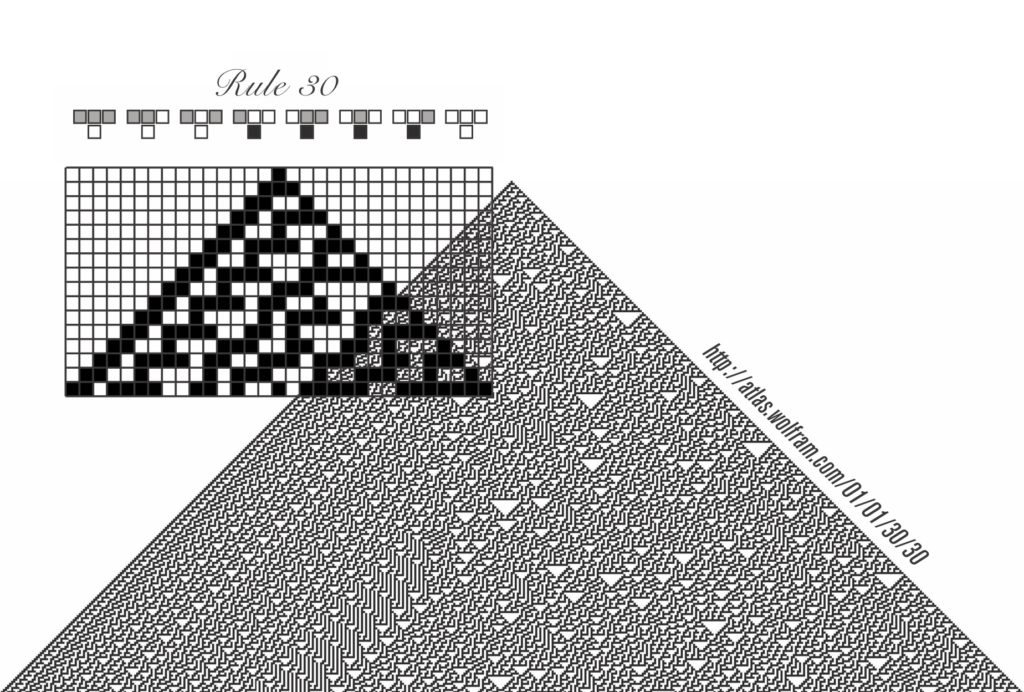
\includegraphics[width=\imsize]{regla30.jpg}
	\caption[ Diagrama que ilustra el patrón generado por la regla 30 del autómata celular (AC) unidimensional.]{  Diagrama que ilustra el patrón generado por la regla 30 del autómata celular (AC)  unidimensional.  Las celdas son coloreadas de acuerdo con su estado anterior en relación a su entorno, asignando tonos más oscuros al estado $1$ y tonos más claros al estado $0$. El eje vertical representa la dimensión temporal, permitiendo visualizar la evolución del patrón a lo largo del tiempo. En la parte superior del diagrama, se presentan las reglas que gobiernan la transición hacia el siguiente estado del autómata, expresadas mediante la fórmula $[\text{celda izquierda} \veebar (\text{celda central} \lor \text{celda derecha})]$. Esta regla específica se denomina Regla $30$ debido a su correspondencia binaria, donde ${00011110}_2$ se representa como el número 30.} \label{fig:regla30}
\end{figure}

\begin{figure}[ht]
	\centering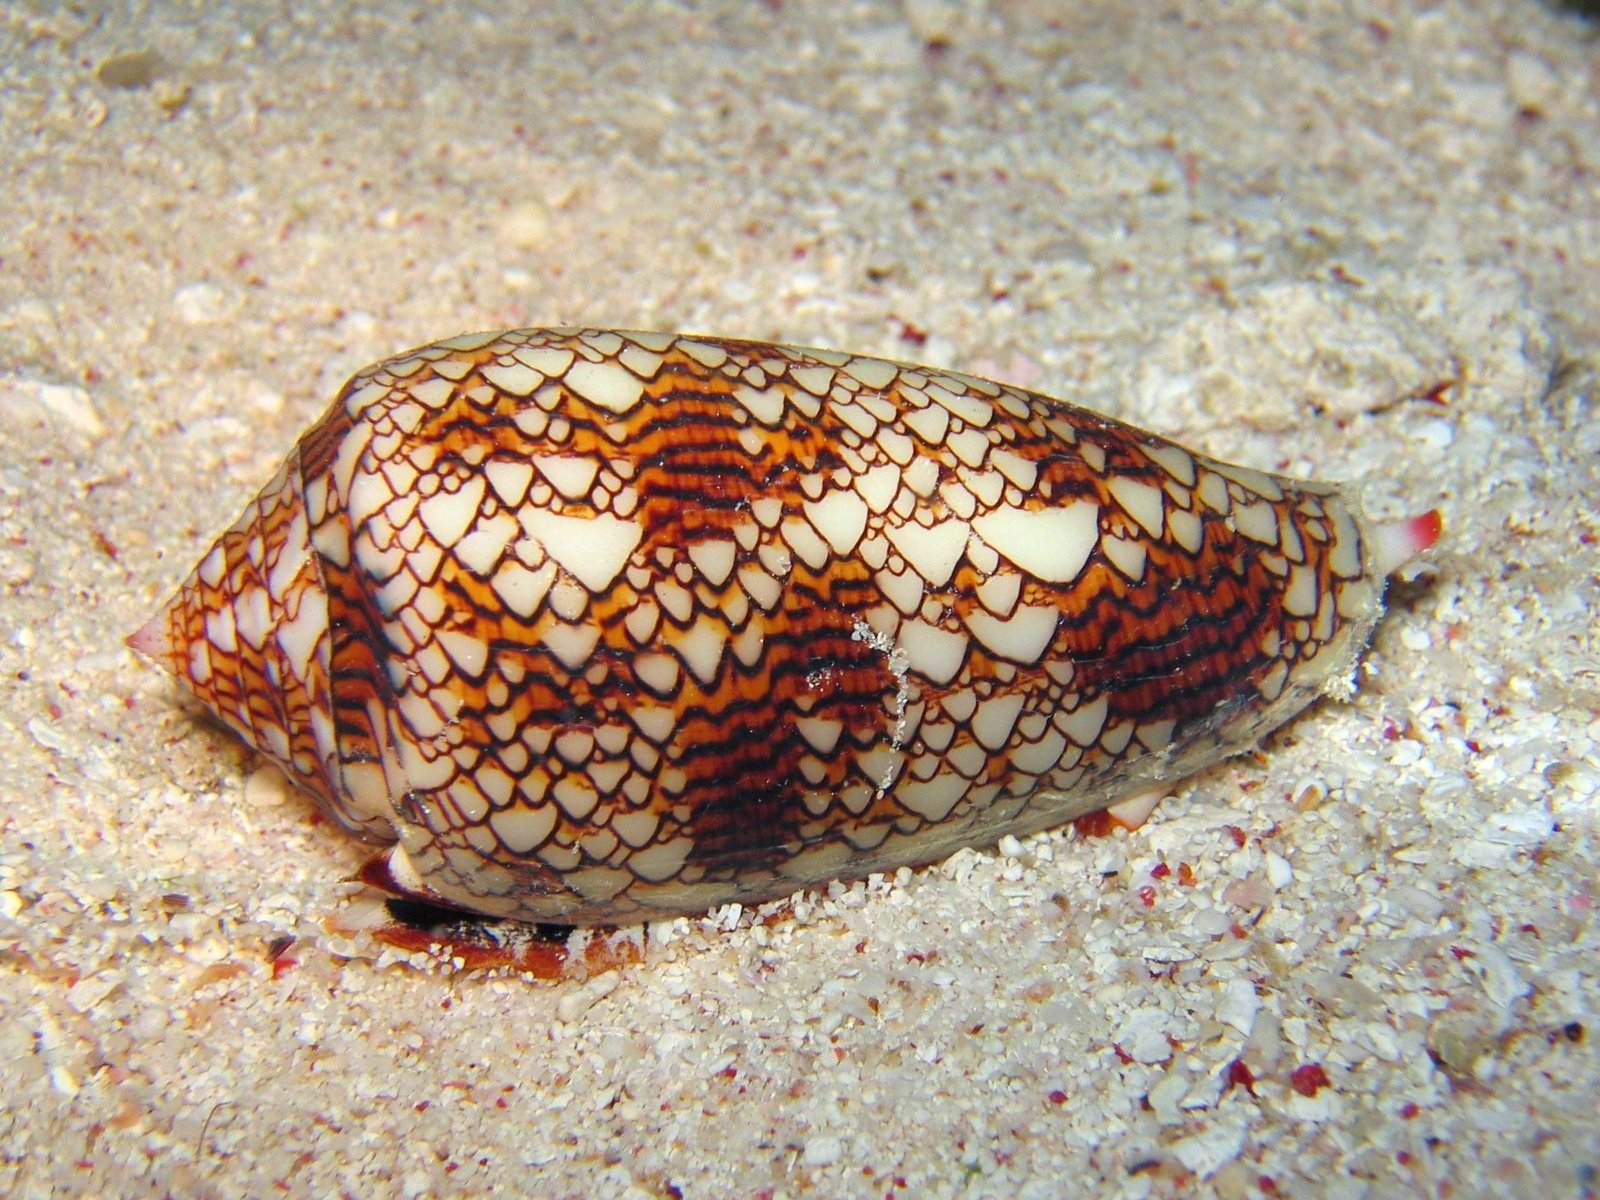
\includegraphics[width=\imsize]{Textile_cone}
	\caption[C Caparazón de Conus textile, una especie presente en las aguas del Indo-Pacífico, que exhibe un patrón de autómata celular con similitudes visuales a la Regla 30.]{ Caparazón de Conus textile, una especie presente en las aguas del Indo-Pacífico, que exhibe un patrón de autómata celular con similitudes visuales a la Regla 30 (Figura adaptada de \protect\cite{ling_english_2005})} \label{fig:conus}
\end{figure}


\subsection{Modelado matemático de autómatas celulares deterministas y estocásticos}\label{sec:SCA}

Los autómatas celulares estocásticos (SCA) pertenecen a la categoría de modelos de red de no equilibrio. Estos modelos se caracterizan por la distribución de celdas (autómatas) en los vértices de una red, donde los enlaces facilitan la interacción y comunicación entre ellas. El análisis de los SCA se centra en los fenómenos que ocurren durante la evolución hacia el equilibrio, así como en aspectos fundamentales como la existencia, número, naturaleza y atracción de las medidas invariantes  de equilibrio \cite{louis_probabilistic_2018}.   En contraste con otras dinámicas asincrónicas, como las ecuaciones diferenciales acopladas o los sistemas de partículas interactuantes, los AC y los SCA pueden definirse directamente en redes infinitas de nodos debido a su naturaleza paralela. Esto evita la necesidad de imponer restricciones a regiones finitas o condiciones adicionales sobre los parámetros para asegurar la existencia del proceso correspondiente. Los AC y SCA se describen mediante el mismo objeto sintáctico, tal como se presenta en la siguiente definición. La distinción entre ellos radica en la forma en que se observa el comportamiento global asociado. Además, los AC deterministas se consideran un caso particular de los SCA. A continuación, se detallan los elementos clave de la configuración matemática de los autómatas:

\begin{itemize}
\item La red  $G$: Se define como un grafo dirigido  $G=(V(G),E(G))$, donde $V(G)$  representa el conjunto de vértices que indican la ubicación de las celdas,  y $E(G)\subseteq V(G)\times V(G)$ es el conjunto de aristas que representan los canales de interacción entre las celdas.
\item El alfabeto $\mathcal{E}$: También conocido como espacio local,, describe los posibles estados o configuraciones que pueden ser adoptados por cada celda. En la mayoría de los autómatas celulares, $\mathcal{E}$ es un conjunto finito con una $\sigma$- álgebra discreta, una topología discreta y una medida uniforme.
\item La vecindad de interacción $\mathcal{N}^I(i)$:  Cada $\mathcal{N}^I(i)\subseteq V(G)$ representa el conjunto de celdas que pueden interactuar con la celda ubicada en $i\in V(G)$. 
\item  El espacio de estado o configuración $\mathcal{S}$:  Representa el estado global de la red de autómatas.   Está equipado con una topología producto y una medida adecuada.  Las configuraciones se denotan como $\mathbf{s}=\left\{s_i:i\in V(G)\right\}$, donde $s_i$ representa el estado de la celda en la ubicación  $i$.
\item Una regla $\mathcal{R}$ que determina la dinámica de los estados de las celdas
\end{itemize}


\subsubsection{Topología de la red y condiciones de contorno}

Los autómatas celulares se definen mediante un grafo $G = (V(G), E(G))$.  El grafo está compuesto por un conjunto $V(G)$ de $N$ nodos (vértices) identificados por el índice $i = 1, \cdots, N$, y un conjunto de aristas $E(G)$ que establecen conexiones entre los nodos, definiendo así la estructura del autómata.  Generalmente, se utiliza un subconjunto finito de la red cuadrada $\mathbb{Z}^2$ como grafo $G$. Esta red cuadrada está compuesta por nodos ubicados en coordenadas enteras en un plano. Los nodos se denominan \textquote{sitios} y la red es invariante ante traslaciones. 

Una arista $(i,j)\in E(G)$ se define como una conexión que tiene origen en el nodo $i$ y destino en el nodo $j$. Se considera una arista saliente de $i$ y entrante en $j$. Decimos que el nodo $i$ es vecino de $j$ si existe una arista entrante de $i$ a $j$, es decir, $(i, j) \in E(G)$. La vecindad de $j$ se define como el conjunto $\mathcal{N}(j) \subseteq V$ que comprende todos los vecinos del nodo $i$.  

\begin{equation}\label{eq:61}
	\mathcal{N}(i)= \left\{j:(i,j)\in E\right\}
\end{equation}

La vecindad también puede ser representada mediante una matriz de adyacencia $\bm{A}$, cuyos elementos están determinados por:

\begin{equation}\label{eq:62}
	a_{ij}=	\begin{cases}
		1, & \text{si} \ \left(i,j\right)\in \mathcal{E}\\
		0, & \text{en caso contrario}
	\end{cases}
\end{equation}

con $i, j = 1,\cdots, N$. Es importante destacar que las conexiones entre nodos pueden ser unidireccionales, lo que significa que no necesariamente son simétricas. Además, es posible tener múltiples redes de conexión entre los mismos nodos, conocidas como multigrafos, representadas mediante diferentes matrices de adyacencia $a_{ij}^{(1)} , a_{ij} ^{(2)}, \cdots$.

Durante los experimentos computacionales en autómatas celulares, se trabaja con redes finitas. Para abordar esta limitación, se establecen condiciones de frontera que determinan la vecindad de las celdas en los bordes de la red. Una estrategia común es la extensión periódica de la red, donde los límites opuestos de la red se conectan. Esto permite que los nodos en los bordes tengan vecinos en el extremo opuesto de la red, creando una estructura anular en una dimensión o un toro en dos dimensiones. Estas condiciones de contorno periódicas se utilizan para aproximar la simulación en una red infinita.  Es importante tener en cuenta que también es posible introducir periodicidades espaciales artificiales en el sistema.

\subsubsection{Vecindario de interacción}

En las redes, se observa una disminución en la fuerza de interacción entre dos nodos a medida que aumenta la distancia en el grafo. Para abordar esta característica, los AC introducen el concepto de vecindad. La vecindad se define como los nodos que están conectados por un número máximo de enlaces, lo cual es crucial en el estudio de los AC, ya que permite evaluar la influencia de los nodos vecinos en el estado de un nodo en particular. En este contexto, se establece el vecindario de interacción $\mathcal{N}^I(i)$ como el conjunto de nodos que afectan el estado del nodo $i$. 

\begin{equation}\label{eq:43}
	\mathcal{N}^I(i) = \left\{j:(i,j)\in E^I\right\}=\left\{j\right\}_{a_{ij}=1}\subseteq G,
\end{equation}

En el caso particular de redes periódicas con condiciones de contorno no periódicas, es necesario considerar la vecindad de interacción en los límites de la red. En las redes bidimensionales cuadradas, se utilizan dos tipos de vecindades comunes: la vecindad de von Neumann y la vecindad de Moore. La vecindad de von Neumann se compone de una celda central y sus cuatro vecinos adyacentes: norte, oeste, sur y este. Por otro lado, la vecindad de Moore incluye los cuatro vecinos adyacentes y los cuatro vecinos diagonales: noreste, noroeste, sureste y suroeste, lo que da un total de nueve celdas.  Estos dos tipos de vecindades estándar se presentan visualmente en la Figura 5.3, proporcionando una representación clara de sus configuraciones en una red bidimensional cuadrada.


\begin{figure}[ht]
	\centering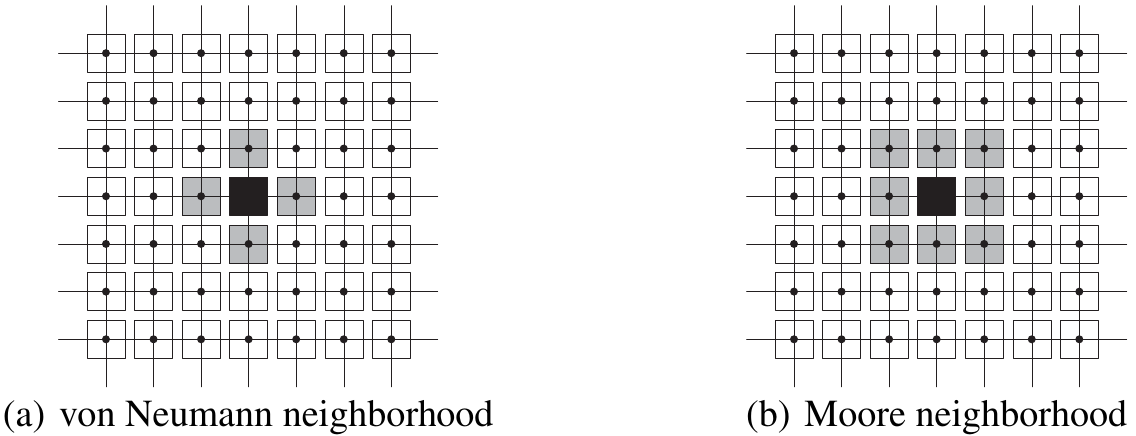
\includegraphics[width=\imsize]{celdas}
	\caption[Ejemplos de vecindades de interacción en una red cuadrada bidimensional. ]{Ejemplos de vecindades de interacción en una red cuadrada bidimensional. Se destacan las celdas grises y negras, que representan los nodos en la red, mientras que la celda negra corresponde al nodo central de interés.} 	\label{fig:celdas}
\end{figure}


\subsubsection{Estados}


Cada nodo $i\in G$ se le asigna un valor de estado $s_i$ tomado de un conjunto finito $\mathcal{E}$ que contiene estados elementales. Esta asignación se define mediante una función de mapeo:

\begin{equation}
	s:G\rightarrow\mathcal{E}.
\end{equation}

El conjunto  $\mathcal{E}$ puede incluir números, símbolos u otros objetos, como células biológicas.  La configuración global del autómata, representada por el vector $\mathbf{s} \in  \mathcal{E}^{N}$, se determina a partir de los valores de estado de todos los nodos en la red, es decir,

\begin{equation}\label{eq:44}
\mathbf{s} \coloneqq \left(s_1,\cdots,s_N\right) = \left(s_i\right)_{i\in G}.
\end{equation}
El espacio de estado $\mathcal{S}$  abarca todas las posibles configuraciones globales y se define como  $\mathcal{S} = \mathcal{E}^{N}$.  Por otro lado, una configuración local se refiere a un vector $\mathbf{s}_\mathcal{M}$   compuesto por los valores de estado de un subconjunto ordenado $\mathcal{M}$   de nodos en la red $G$

\begin{equation}\label{eq:45}
\mathbf{s}_\mathcal{M} \coloneqq \left(s_1,\cdots,s_\mathcal{M}\right)=(s_i)_{i\in\mathcal{M}}, \ \mathcal{M} \subset G.
\end{equation}

La notación $\mathbf{s}\mid\mathcal{M}=\mathbf{s}_\mathcal{M}\in\mathcal{S}\mid\mathcal{M}$  se utiliza para indicar la restricción de la configuración global  $\mathbf{s}$ 
al conjunto $\mathcal{M}$.  Además, la configuración local en relación al entorno de interacción  $\mathcal{N}^I( )\subseteq G$ de un nodo  $i$ se denota como $\mathbf{s}_{\mathcal{N}(i)} \in \mathcal{S}_{\mathcal{N}(i)} \coloneqq \mathcal{S}\mid \mathcal{N}^I(i)$.

\subsection{Dinámica del sistema}\label{sec:dinamica_automata}

La dinámica de un autómata celular está determinada por una regla de transición local, representada por $\mathcal{R}$, que determina el estado futuro de cada nodo en función de su configuración de vecindad de interacción. Formalmente, esta regla se define como:


\begin{align}\label{eq:46}
	\mathcal{R}&:\mathcal{E}^\nu\rightarrow\mathcal{E}, \quad \text{donde} \  \nu = \left| \mathcal{N}_n^I\right|.\\
\end{align}


Donde $ \nu = \left| \mathcal{N}_n^I\right|$ representa la cardinalidad de $\mathcal{N}_n^I$. Se considera que la regla $\mathcal{R}$  es espacialmente homogénea, lo que significa que no depende explícitamente de la posición del nodo $i$. Sin embargo, se pueden introducir variaciones para permitir la falta de homogeneidad espacial y temporal en la regla. Por ejemplo, es posible incorporar reglas dependientes del tiempo, como alternar entre dos reglas en pasos de tiempo pares e impares, tal como se utiliza en modelos de autómatas celulares para casos como la percolación dirigida o la dinámica de espín de Ising. Aunque en general se asume que la regla de transición es espacialmente homogénea.


En un autómata celular determinista, la regla local es determinista y genera un único estado siguiente para cada nodo. Por lo tanto, bajo condiciones iniciales fijas, la evolución futura del autómata es predecible y está determinada de manera única.

Por otro lado, cuando las actualizaciones son aleatorias, se tiene un autómata celular estocástico que sigue un proceso de Markov. En cada paso de tiempo, el estado de cada nodo se actualiza aleatoriamente e independientemente de los demás, siguiendo una distribución de probabilidad que depende del patrón actual de símbolos en una colección finita de sitios vecinos \cite{marcovici_ergodicity_2019}. En un autómata celular estocástico, la regla de transición local se define de la siguiente manera:

\begin{equation}\label{eq:47}
\mathcal{R}\left(\mathbf{s}_{\mathcal{N}(i)}\right) = \begin{cases}
	z^1& \text{con probabilidad} \ W\left(\mathbf{s}_{\mathcal{N}(i)}\rightarrow z^1\right),\\
	\vdots\\
	z^{\left\| \mathcal{E}\right\|} & \text{con probabilidad} \ W\left(\mathbf{s}_{\mathcal{N}(i)}\rightarrow z^{\left\| \mathcal{E}\right\|} \right),
\end{cases}
\end{equation}

donde $z^j \in \mathcal{E} := \left\{z^1,\cdots,z^{\left\|\mathcal{E} \right\| }\right\}$ y $W\left(\mathbf{s}_{\mathcal{N}(i)}\rightarrow z^j\right)$ es la probabilidad de transición independiente del tiempo.  Esta probabilidad indica la posibilidad de que el nodo alcance el estado elemental $z^j$, dada la configuración de vecindad $\mathbf{s}_{\mathcal{N}(i)}$ en ese momento. Es importante destacar que esta probabilidad de transición debe satisfacer ciertas condiciones:

\begin{equation}\label{eq:48}
W:\mathcal{E}^\nu\times\mathcal{E}\rightarrow[0,1] \quad \text{y} \quad  \sum_{j=1}^{\left\| \mathcal{E}\right\| }{W\left(\mathbf{s}_{\mathcal{N}(i)}\rightarrow z^j\right)}=1, \quad \mathbf{s}_{\mathcal{N}(i)}\in\mathcal{E}^\nu,z^j\in\mathcal{E}.
\end{equation}

Es relevante mencionar que cualquier regla local determinista puede considerarse como un caso especial de una regla probabilística, donde la probabilidad de transición es igual a $1$ para el estado objetivo y $0$ para los demás estados, es decir

\begin{equation}\label{eq:49}
	W\left(\mathbf{s}_{\mathcal{N}(i)}\rightarrow z^j\right)=1 \quad \text{y} \quad W\left(\mathbf{s}_{\mathcal{N}(i)}\rightarrow z^l\right)=0 \quad \forall l\neq j,z^j,z^l\in\mathcal{E}.
\end{equation}


Los autómatas celulares estocásticos son una generalización valiosa en el campo de los sistemas complejos, debido a su capacidad para ajustar los parámetros de una regla en un rango continuo de valores, a pesar de la naturaleza discreta inherente a los autómatas celulares.   En un autómata celular con actualización síncrona, la regla local se aplica simultáneamente a cada nodo de la red antes de que los nuevos estados influyan en otros nodos. Esto implica que la dinámica global está determinada por una función global  $\mathcal{R}_g:\mathcal{S}\rightarrow\mathcal{S}$ tal que para cada configuración global $\mathbf{s} \in \mathcal{S}$,

\begin{equation}\label{eq:50}
	\mathcal{R}_g(\mathbf{s}(i))=\mathcal{R}\left(\mathbf{s}_{\mathcal{N}(i)}\right) \quad \forall i\in G.
\end{equation}

En consecuencia, la dinámica global está completamente definida por la regla local $\mathcal{R}$.   Denotamos la configuración global en pasos de tiempo posteriores $t \in \mathbb{N}_0$ como  $\mathbf{s}(t)= (s_1(t),\cdots, s_N( t)) \in \mathcal{S}$, donde $s_i(t) \in \mathcal{E}$ representa el estado del nodo  $i$ en el tiempo $t$.  La configuración local del nodo $i$ en el tiempo $t$  está dada por $\mathbf{s}_{\mathcal{N}(i)} (t) \in  \mathcal{S}_{\mathcal{N} (t)}$.   Para cada configuración global inicial 
 $\mathbf{s} (0) \in \mathcal{S}$ en el tiempo $t=0$,  el desarrollo temporal del sistema se describe mediante la siguiente relación:


\begin{equation}\label{eq:51}
\mathbf{s}(t+1)=\mathcal{R}_g(\mathbf{s}(t)),
\end{equation}

La dinámica de un estado $s_i(t)$ se determina mediante la regla local $\mathcal{R}$,  es decir:
\begin{equation}\label{eq:52}
s_i(t+1)=\mathcal{R}\left(\mathbf{s}_{\mathcal{N}(i)}(t)\right).
\end{equation}

En otras palabras, el estado del nodo $s_i( t )$ depende de los estados anteriores de los nodos de entrada.  Dado que el número de configuraciones posibles es finito para una red finita, cualquier condición inicial eventualmente conduce a un ciclo temporal periódico en un autómata celular determinista. En el caso de los autómatas celulares estocásticos, se puede entender su evolución como una cadena de Markov, donde los elementos de la matriz de transición se obtienen multiplicando las probabilidades de transición locales. La dinámica global de los autómatas celulares finitos se puede visualizar mediante un grafo de transiciones globales, donde cada nodo representa una configuración única del autómata celular y las aristas que los conectan representan las transiciones globales entre las configuraciones.


En extensiones de los modelos de autómatas celulares, se permite la actualización asíncrona y no se limita a vecindarios finitos. En este caso, la regla local se aplica de forma independiente a cada nodo, lo que implica que el nuevo estado de un nodo afecta el cálculo de los estados en celdas vecinas. Estas diferencias en la actualización asíncrona tienen implicaciones significativas en la dinámica y los patrones generados por los autómatas celulares. Se han propuesto y analizado varios algoritmos de actualización asíncrona \cite{schonfisch_synchronous_1999,cornforth_ordered_2005,fates_guided_2013}. Cabe destacar que varios estudios han implementado modelos asíncronos y han observado que su comportamiento difiere de los modelos síncronos. Sin embargo, Nehaniv demostró que es posible emular con precisión el comportamiento de un autómata celular síncrono mediante una sencilla modificación del autómata celular asíncrono utilizando un método general \cite{nehaniv_asynchronous_2011}.



\section{Modelos de AC de sistemas excitables}\label{sec:medios_excitables}

En el apartado \cref{sec:mediosexcitables}  se discute la naturaleza de los medios excitables, los cuales son sistemas extendidos de no equilibrio. Estos sistemas exhiben estados uniformes que son linealmente estables, pero que pueden ser perturbados por estímulos finitos. Los medios excitables consisten en elementos acoplados, cada uno de los cuales muestra una dinámica estable hasta que se alcanza un umbral específico. La evolución de estos elementos en el espacio de fase se manifiesta como ondas viajeras en el tiempo real. La capacidad de respuesta a las perturbaciones es una característica fundamental de los elementos excitables. Cuando se supera un umbral determinado, una perturbación excitará un elemento inactivo, que luego volverá a la inactividad tras un tiempo característico, sin importar la magnitud de la perturbación. Estas ondas excitables ilustran de manera sorprendente la ruptura de simetría espontánea y la organización espacio-temporal en sistemas físicos y químicos.

La investigación experimental y numérica de los sistemas excitables tiene una larga trayectoria. Por lo general, se utiliza un sistema de ecuaciones diferenciales parciales para modelar el mecanismo de reacción-difusión subyacente. Si bien estos modelos suelen ser efectivos, la implementación de métodos numéricos adecuados puede ser compleja y las simulaciones computacionales pueden requerir mucho tiempo, especialmente en el caso de sistemas tridimensionales.

En los últimos años, los modelos basados en autómatas celulares han ganado popularidad como una alternativa para el modelado de dichos sistemas. Estos modelos presentan ventajas significativas, como un menor costo computacional, una mayor flexibilidad y una configuración más sencilla. Los modelos de autómatas celulares para medios excitables buscan simplificar el sistema al máximo, donde cada unidad excitante puede asumir un número finito de estados. La dinámica de actualización de cada unidad excitante depende tanto de su estado actual como del estado de sus vecinos \cite{sinha_patterns_2019}.



En 1946, Wiener y Rosenblueth dieron los primeros pasos hacia la comprensión de los medios biológicos excitables al utilizar autómatas celulares. Su estudio se enfocó en explicar las arritmias cardíacas generadas por las ondas espirales, y propusieron los estados refractario, quiescente y excitado como base para entender el comportamiento de dichos medios \cite{wiener_mathematical_1946}.  Posteriormente, en 1978, Greenberg y Hastings llevaron a cabo un estudio fundamental en el que presentaron un modelo de autómatas celulares con una dinámica trifásica, cíclica y excitante para el modelado de medios excitables. Este modelo, conocido como el modelo de autómatas celulares de Greenberg-Hastings (GHCA) \cite{greenberg_spatial_1978}, ha demostrado ser un marco fructífero para el estudio y análisis de dichos sistemas. En particular, se ha utilizado con éxito para modelar las reacciones de Belousov-Zhabotinsky, que representan un ejemplo prototípico de medios excitables, y ha proporcionado información valiosa sobre estos sistemas. En general, el modelo GHCA pertenece a una clase más amplia de autómatas celulares con dinámica local excitante y cíclica, y se ha implementado en modelos computacionales para estudiar fenómenos biológicos, como los patrones espaciotemporales de los ritmos cardíacos, las ondas cerebrales macroscópicas y los procesos epidémicos  \cite{hadeler_cellular_2017}.



\subsection{Modelo  de Greenberg-Hastings}\label{sec:modeloGH}


El modelo Greenberg-Hastings fue desarrollado por Greenberg y Hastings como una simplificación del modelo Fitzhugh-Nagumo, que describe la excitación nerviosa. Mientras que el modelo Fitzhugh-Nagumo exhibe un comportamiento periódico cuando la entrada dendrítica supera un umbral  (ver \cref{modelo_Fitzhugh-Nagumo}), el modelo Greenberg-Hastings se centra en capturar esta dinámica de manera más simplificada y abstraída. El modelo Fitzhugh-Nagumo se compone de dos ecuaciones diferenciales acopladas, que representan el estado del sistema. En su mayoría, el sistema permanece en las dos partes estables del manifold lento, y los saltos a través del manifold rápido son breves y pueden ser desestimados. Al discretizar el tiempo y analizar la solución de las ecuaciones en puntos de tiempo discretos equidistantes, se observa que la célula sigue una secuencia discreta: primero avanza por la rama activada del manifold lento y luego por la rama refractaria (ver  \Cref{fig:Nagumo}). Se utiliza el estado 0 para denotar el estado de reposo, y los estados se numeran en orden ascendente \cite{hadeler_cellular_2017}. Dentro del manifold lento, encontramos varios estados excitados, que se denominan $K$, junto con $\kappa - K$ estados refractarios. Además, se incluye el estado de reposo, lo que da un total de $\kappa + 1$ estados posibles. Estos estados se recorren de forma cíclica, siguiendo la secuencia:

\begin{equation}
	\underbrace{0}_{\text{quiescente}}\to \underbrace{1\to2\to\cdots K-1\to K}_{\text{excitado}}\to\underbrace{K+1\to K+2\to\cdots \kappa-1\to \kappa}_{\text{refractario}}\to\underbrace{0}_{\text{quiescente}}.
\end{equation}

\begin{figure}[ht]
	\centering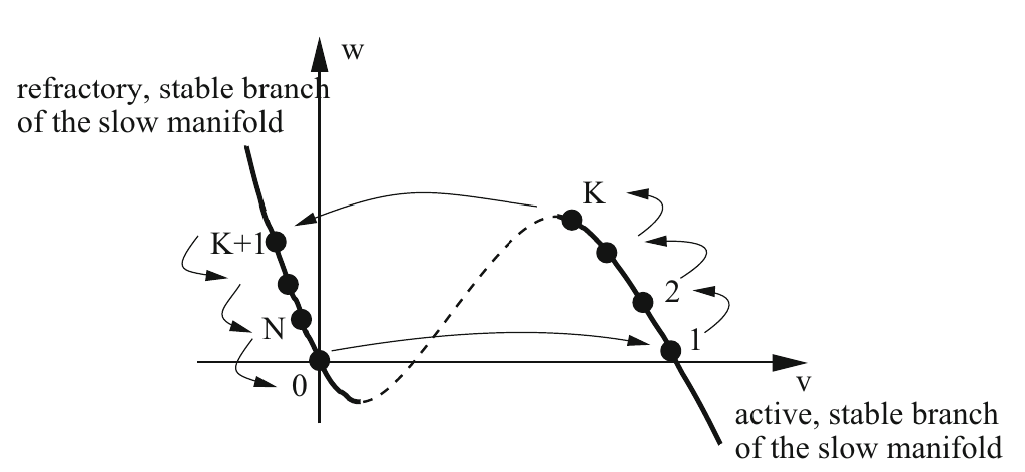
\includegraphics[width=\imsize]{Nagumo.png}
	\caption[Reducción del modelo Fitzhugh-Nagumo a un sistema discreto. ]{Reducción del modelo Fitzhugh-Nagumo a un sistema discreto. El estado sigue la parte excitada y luego la parte refractaria del manifold lento. Utilizando pasos de tiempo discretos, el sistema recorre los estados marcados con puntos negros. (adaptada de \protect\cite{hadeler_cellular_2017})}\label{fig:Nagumo}
\end{figure}

Para proporcionar una descripción completa del modelo, se deben tener en cuenta las siguientes características:

\begin{enumerate}
	\item  Una vez que una celda alcanza el estado $1$, sigue una secuencia determinista de estados ascendentes  $2,\cdots,\kappa$, independientemente de las celdas vecinas. En cada paso de tiempo, el estado se incrementa en uno, hasta que alcanza el estado $\kappa + 1$, que se reduce a $0$ mediante el módulo $\kappa + 1$. El acoplamiento entre las células vecinas es tan débil que solo el estado de reposo puede ser afectado por las células adyacentes.
	\item Si una celda está en estado de reposo, la transición $0\to1$  ocurre cuando al menos $\theta$ celdas en la vecindad de von Neumann se encuentran en un estado excitado $1,\cdots,K$ . 
\end{enumerate}

\begin{definitionT}[Autómata Celular de Greenberg-Hastings]
	Consideremos $G=\mathbb{Z}^2$ como la cuadrícula y $\mathcal{N}_4^I(i)$  como la vecindad de von Neumann. Sean $K,\kappa,\theta, \in \mathbb{N}$, donde $0<K<\kappa$ y  sea $\mathcal{E}=\left\{0,\cdots,\kappa\right\}$.   La dinámica de un estado $s_i(t)$ se describe mediante la siguiente ecuación discreta:
	\begin{align}\label{eq:53}
	s_i(t+1)&= \mathcal{R}(\mathbf{s}_{\mathcal{N}(i)}(t)) \\	
		&=\begin{cases}
			(i+1) \mod (\kappa+1) & \text{si} \ s_i(t)=i\in\mathcal{E}\backslash \left\{0\right\},\\
			0 & \text{si} \ s_i(t)=0 \land \# \left\{ j \in \mathcal{N}^I(i):  1 \leq s_j \leq K\right\}<\theta,\\
			1 & \text{si} \ s_i(t)=0 \land \# \left\{ j \in \mathcal{N}^I(i):  1 \leq s_j \leq K\right\}\geq\theta,
		\end{cases}
	\end{align}
	
	este sistema dinámico discreto se denomina autómata celular de AC de Greenberg-Hastings. 
\end{definitionT}

Este sistema  ha demostrado converger hacia un estado estacionario de oscilaciones espaciotemporales o hacia un punto fijo sin actividad en el sistema.   Para facilitar su análisis, asignamos colores a los $\kappa + 1$ posibles estados en cada celda. La \Cref{fig:gh} muestra ejemplos representativos de la evolución del modelo GHCA en una cuadrícula de tamaño $240\times240$ , con diferentes valores de $\theta$ y $\kappa$. En estos experimentos, partimos de una configuración inicial conocida como \textquote{sopa primordial}, donde los colores iniciales de las celdas son independientes y tienen igual probabilidad de tomar cualquiera de los $\kappa + 1$ valores posibles.


\begin{figure}[h!]
	\centering
	\begin{subfigure}{0.45\linewidth}
		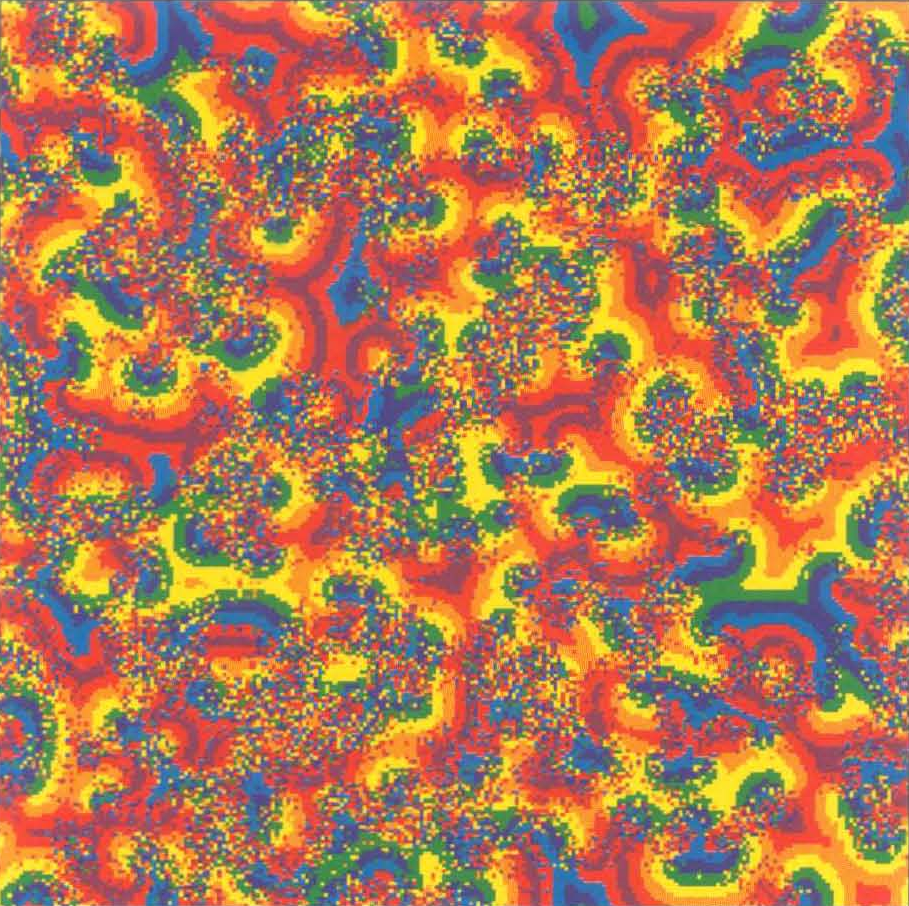
\includegraphics[width=\linewidth]{gh1} 
		\caption{$\theta=6,\kappa=8$}
		\label{fig:gh1a}
	\end{subfigure}\hfill
	\begin{subfigure}{0.45\linewidth}
		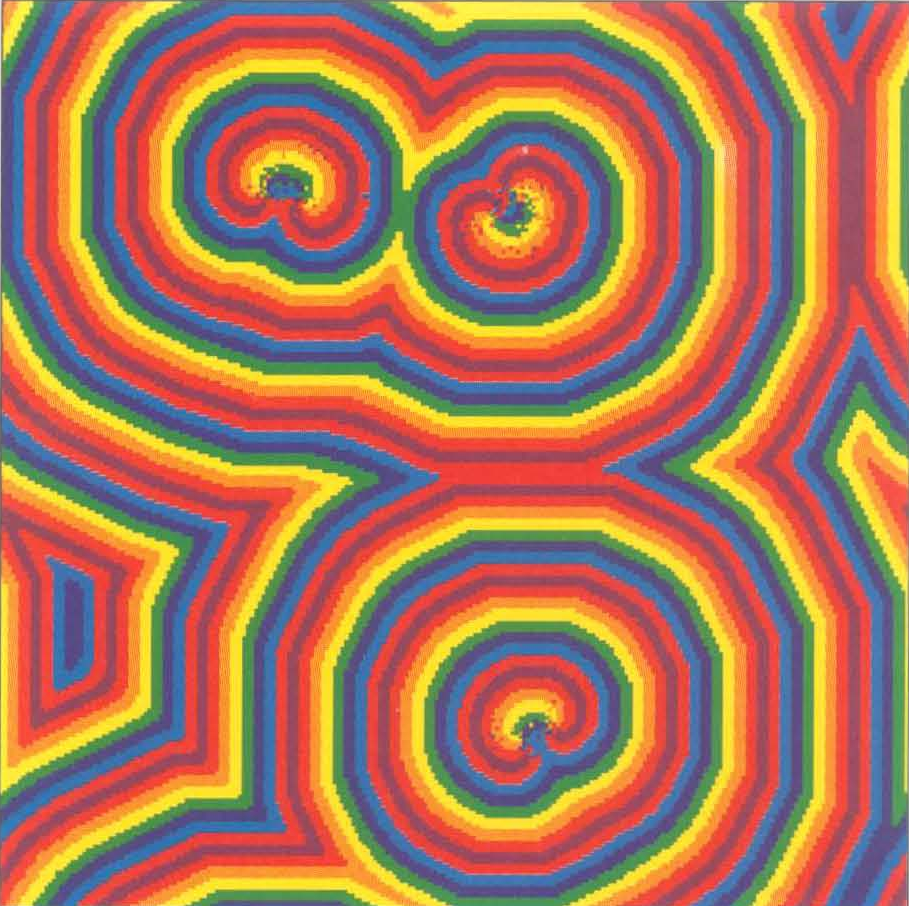
\includegraphics[width=\linewidth]{gh2}
		\caption{$\theta=7,\kappa=8$}
		\label{fig:gh1b}
	\end{subfigure}
	
	\begin{subfigure}{0.45\linewidth}
		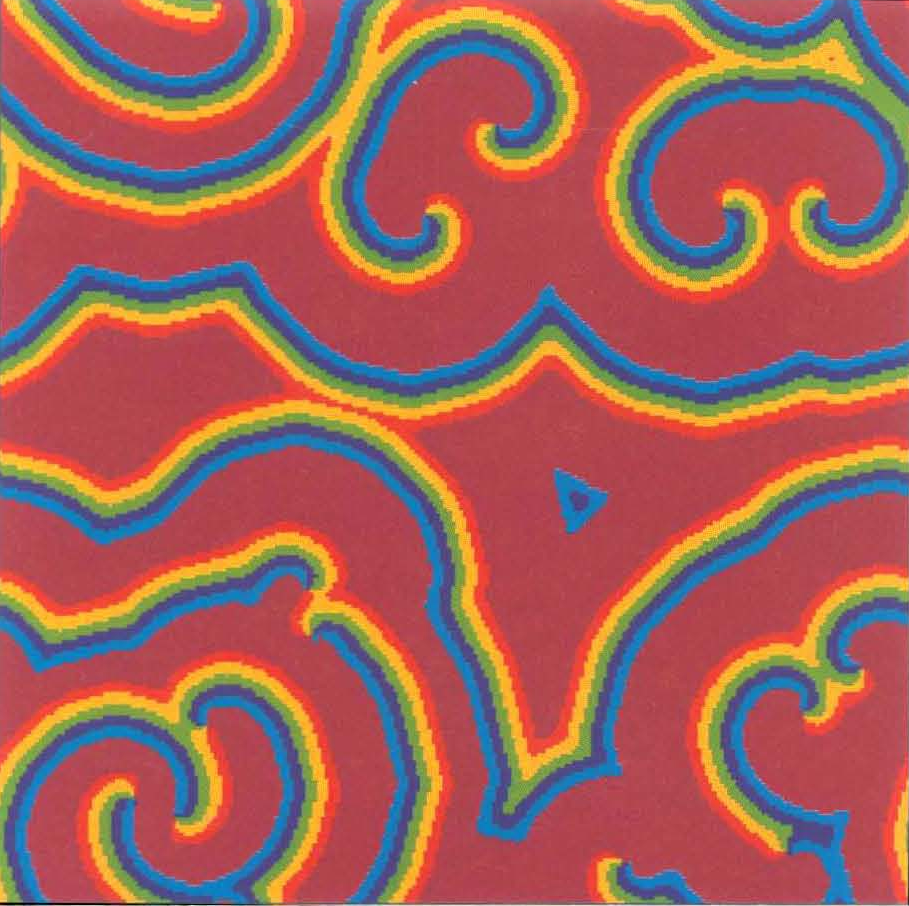
\includegraphics[width=\linewidth]{gh3}
		\caption{$\theta=9,\kappa=6$}
		\label{fig:gh1c}
	\end{subfigure}\hfill
	\begin{subfigure}{0.45\linewidth}
		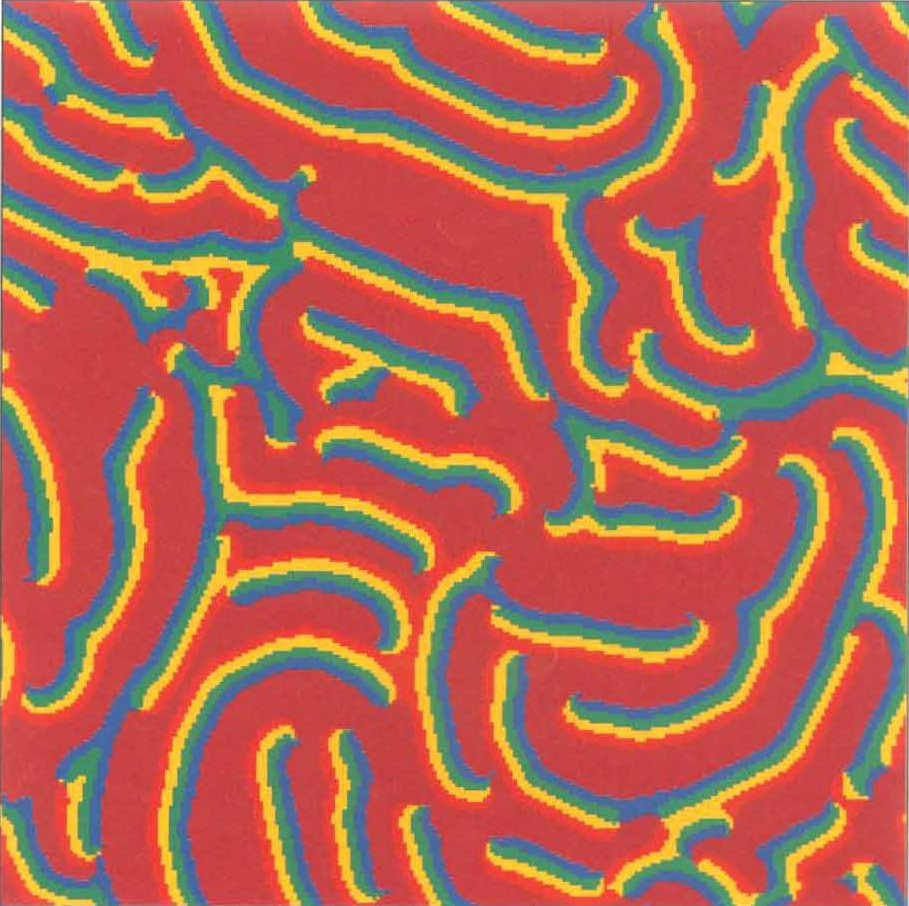
\includegraphics[width=\linewidth]{gh4}
		\caption{$\theta=10,\kappa=5$}
		\label{fig:ghd}
	\end{subfigure}
	\caption[Instantáneas representativas que ilustran la evolución del modelo de Greenberg-Hastings en una cuadrícula de tamaño $240\times240$, con variaciones en los valores de $\theta$ y $\kappa$. ]{Instantáneas representativas que ilustran la evolución del modelo de Greenberg-Hastings en una cuadrícula de tamaño $240\times240$, con variaciones en los valores de $\theta$ y $\kappa$. Los estados iniciales se generaron asignando colores de manera aleatoria a cada celda con la misma probabilidad. Las instantáneas fueron capturadas después de $100$ pasos. Se implementaron condiciones de contorno periódicas para garantizar la consistencia, lo que implica que los bordes opuestos son idénticos (Imágenes obtenidas de \protect\cite{durrett_asymptotic_1993}).}
	\label{fig:gh}
\end{figure}





\section{Dinámica critica en el C elegans}

En el campo de la neurociencia actual, uno de los desafíos más relevantes consiste en comprender cómo surge y se organiza la actividad neuronal compleja a partir de las interacciones entre las neuronas. En los últimos años, se ha prestado mayor atención a este desafío a medida que se han desarrollado y mejorado las técnicas experimentales para registrar simultáneamente la actividad de múltiples neuronas, lo que proporciona conjuntos de datos valiosos para su análisis. Se ha observado que, incluso en ausencia de estímulos externos, la actividad de la red neuronal se organiza en patrones espacio-temporales complejos que reflejan, hasta cierto punto, la arquitectura subyacente de la red. Estos patrones dinámicos muestran similitudes con los sistemas termodinámicos que experimentan una transición de fase de segundo orden, lo que respalda la hipótesis de que el cerebro funciona como un sistema autoorganizado en un estado crítico. Un experimento relevante realizado por Kato et al. combinó tecnologías avanzadas, como la obtención de imágenes de calcio a nivel de una sola célula, para registrar la actividad neuronal en todo el cerebro de un  gusano Caenorhabditis elegans  inmovilizado  en un pequeño canal \cite{kato_global_2015}.  Los resultados obtenidos demostraron una actividad dinámica y coordinada en una amplia proporción de las neuronas cerebrales. Además, Kaplan et al. realizaron experimentos adicionales que confirmaron y ampliaron estos hallazgos  \cite{kaplan_nested_2020}.


Asimismo, es fundamental investigar la relación entre la actividad neuronal y la arquitectura de la red. Estudios previos han demostrado que la complejidad de la arquitectura determina las interacciones complejas entre las diferentes áreas del cerebro \cite{galan_how_2008}. Se ha observado que las conexiones locales densas y las conexiones de largo alcance escasas tienden a generar un comportamiento complejo a gran escala. Sin embargo, la mayoría de estos estudios se han centrado en un nivel macroscópico, describiendo las interacciones entre áreas cerebrales o en el contexto general de arquitecturas de redes complejas pero que no abarca todo el sistema nervioso de forma global, lo que limita su aplicabilidad y generalización.


En esta tesis de doctorado, se propone un enfoque novedoso para abordar estos desafíos, integrando la dinámica neuronal a nivel de sinapsis en una arquitectura que abarque todo el cerebro. Para lograrlo, se utilizará el conectoma completo de ambos sexos de Caenorhabditis elegans. Este enfoque supera las limitaciones de los modelos actuales, que se basan en regiones cerebrales macroscópicas y emplean una dinámica de red basada en un número reducido de neuronas. Además, al aprovechar las diferencias en el sistema nervioso entre los sexos de Caenorhabditis elegans, será posible investigar la relación entre la arquitectura de la red y la actividad espontánea a nivel global.  Para abordar este problema, se empleará un enfoque de modelado estocástico, ampliamente utilizado en la neurociencia matemática. La actividad neuronal presenta un carácter estocástico, por lo que la interacción entre la excitabilidad neuronal y el estocasticismo constituye un aspecto central en esta investigación. En ausencia de estímulos externos, la red neuronal estará influenciada por fluctuaciones intrínsecas y aleatorias, modeladas como actividad espontanea. Estas fluctuaciones surgirán de las variaciones en los eventos de apertura y cierre de los canales iónicos, así como de la liberación sináptica espontánea y otras fuentes de variabilidad biológica. Estas corrientes aleatorias desencadenarán tasas moderadas de activación en las neuronas individuales, las cuales se propagarán a través de la red neuronal gracias a las interacciones sinápticas.





\subsection{Modelo de dinámica neuronal estocástica en el cerebro de C. elegans }\label{sec:modelocritico}


En esta sección, se abordará la construcción de un modelo de red neuronal basado en autómatas celulares estocásticos para simular el comportamiento de las neuronas de disparo. Con el fin de lograr una representación adecuada de la dinámica real de estas neuronas, es crucial comprender  su fisiología, lo que permitirá desarrollar un modelo más realista. Por lo tanto, se iniciará este estudio profundizando en la fisiología de las neuronas de disparo, centrándonos en los detalles del potencial de acción, tal como se muestra en la \cref{fig:spikeautomata}.   Previo a esta sección, se estableció en el \cref{sec:modelo_dinamica_neuronal} que las neuronas de disparo pueden clasificarse en tres estados principales: el estado quiescente, corresponde al período de reposo, en el cual el potencial de membrana neuronal se mantiene estable en a \qty{-70}{\milli\volt}; el estado excitado, cuando el potencial de membrana se eleva desde un umbral de alrededor de \qty{-55}{\milli\volt} hasta \qty{40}{\milli\volt} (potencial de inversión del sodio), para luego retornar a  \qty{-80}{\milli\volt} (potencial de inversión del potasio) en aproximadamente  \qty{1}{\milli\second}; Por último, el estado refractario se caracteriza por el retorno gradual del potencial de membrana hacia el estado de reposo. Con base en los argumentos expuestos en el \cref{sec:modeloGH}, se representa estos estados mediante una variable de estado discreta,  $\mathbf{s} = \{Q, E, R\}$. En esta notación,  $s_i = Q$ representa el estado quiescente, $s_i = E$ el estado excitado y $s_i = R$ corresponde al período refractario. Es importante destacar que la neurona puede disparar únicamente en el estado quiescente ($s_i = Q$), no durante el período refractario. Por lo tanto, se deben considerar tres transiciones de estado: $Q\to E$ , que depende de las conexiones que esta neurona tenga con otras, y $E\to R$, $R\to Q$, que corresponden a decaimientos simples.



\begin{figure}[ht]
	\centering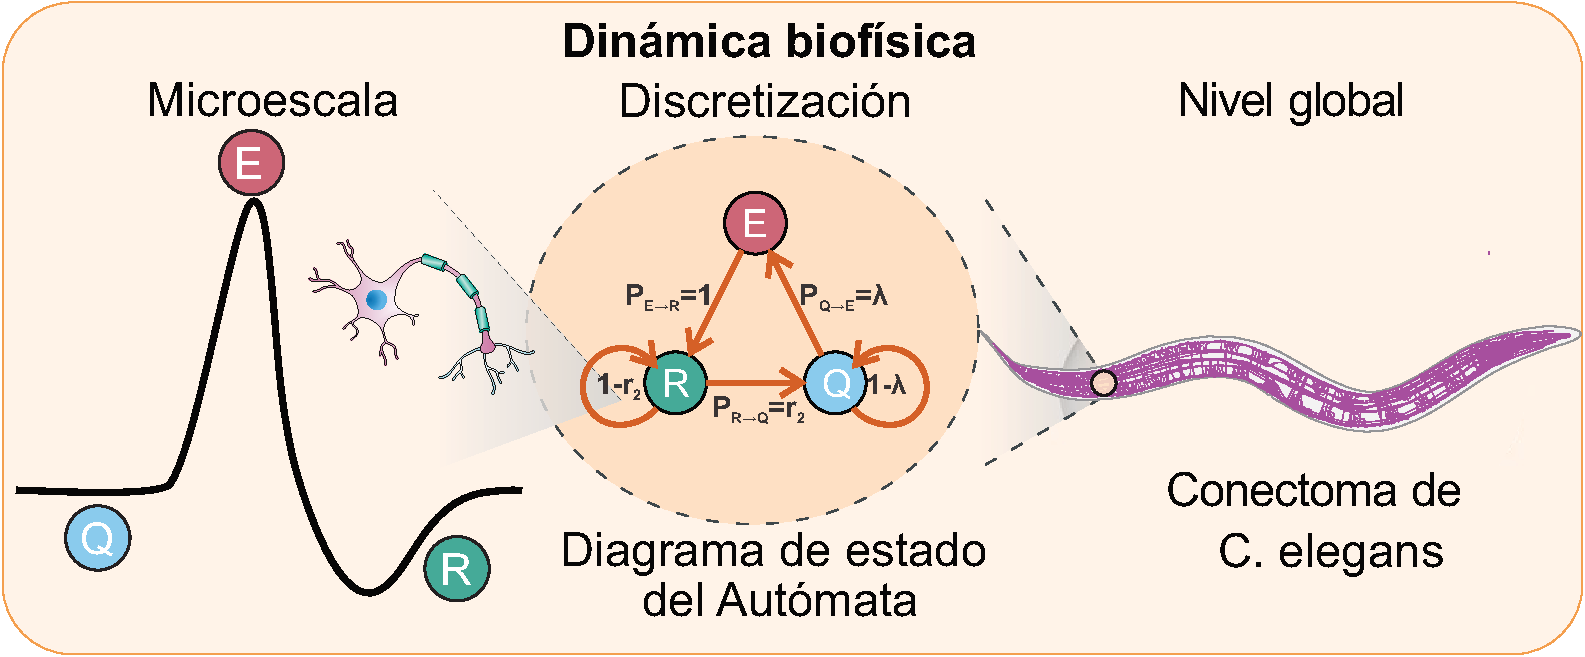
\includegraphics[width=\imsize]{modelo}
	\caption[Modelado de la función de la red cerebral.]{ Modelado de la función de la red cerebral. En el panel izquierdo, se presenta el esquema del potencial de acción de una neurona real, el cual sirve como fundamento del modelo neural. En el panel central, se exhibe el diagrama de estados de los autómatas finitos que representan a las neuronas en el modelo. Estos autómatas pueden adoptar tres estados diferentes: quiescente (Q), excitado (E) o refractario (R). La discretización del potencial de acción, explicada previamente, es esencial para definir estos estados. Las neuronas activas (E; en rojo) emiten ráfagas de potenciales de acción antes de ingresar al estado refractario (R; en verde) durante un período determinado por la probabilidad de $1-r_2$, donde $r_2$ representa la probabilidad de que una neurona pase al estado quiescente. Por otro lado, las neuronas quiescentes (Q; en azul) también desempeñan un papel significativo. Pueden generar potenciales de acción espontáneamente con una probabilidad $r_1$, o ser reclutadas en una ola de actividad por otras neuronas activas si la suma de sus pesos supera un umbral $T$. La probabilidad de esta reclutación, representada en el diagrama de estados mediante el parámetro $\lambda=1-\left[1-r_1\right]\left[1-\Theta\left(\sum_{j=1}^{k_{in,i}}W_{ji}\delta_{s_j,1}-T\right)\right]$, es esencial para la dinámica del modelo y se basa en las características específicas de cada estado neuronal. Para simular la actividad a gran escala del cerebro completo, los autómatas se incorporan al conectoma del C. elegans, lo que permite la aparición de interacciones complejas entre las neuronas y da lugar a una dinámica global compleja, ilustrada en el panel derecho. Cada una de estas neuronas sigue la dinámica presentada en el diagrama de estados y contribuye al comportamiento del modelo a gran escala (La figura ha sido adaptada de las referencias \cite{lynn_physics_2019, jjfroehlich_english_2022}).}\label{fig:spikeautomata}
\end{figure}


Para representar esta abstracción discreta de la fisiología de las neuronas de disparo, se adaptará el modelo computacional del autómata celular de Greenberg-Hastings descrito en el \cref{sec:modeloGH}. En este estudio, se seguirá de cerca la implementación propuesta por \cite{haimovici_brain_2013}.  Las conexiones en el modelo se basarán en la matriz de adjacencia del conectoma del C. elegans, tanto para los sexos hermafrodita como macho, construida por Cook et al \cite{cook_whole-animal_2019}. Para obtener una descripción detallada del conectoma y su derivación a partir de la microscopía electrónica en serie, se puede consultar el apartado 1.1. En resumen, el conectoma del hermafrodita consta de 460 nodos (302 neuronas, 132 músculos y 26 órganos terminales no musculares), mientras que el conectoma del macho cuenta con 579 nodos (385 neuronas, 155 músculos y 39 órganos terminales no musculares). Dichos conectomas presentan un total de 4,887 conexiones químicas (o dirigidas) y 1,447 conexiones gap junction (o no dirigidas) en el caso del hermafrodita, y 5,315 conexiones químicas y 1,755 conexiones gap junction en el caso del macho. Los pesos de estas conexiones, denotados como wij, corresponden al número total de secciones seriales de conectividad EM, teniendo en cuenta tanto el número como el tamaño de las sinapsis. Cabe mencionar que este modelo se limitará únicamente a las conexiones químicas del conectoma, ya que nuestro objetivo es enfocarnos exclusivamente en las sinapsis entre neuronas. Sin embargo, es importante destacar que el modelo es lo suficientemente flexible como para incorporar fácilmente las conexiones eléctricas si se desea (ver, por ejemplo, \cite{protachevicz_how_2018}).

Además de las conexiones, el modelo también tendrá en cuenta otros aspectos relevantes desde el punto de vista neurofisiológico, que pueden tener implicaciones dinámicas significativas.  Entre ellos, se destaca la incorporación de una probabilidad de excitación espontánea $r_1$ en cada neurona, lo que implica que existe una pequeña posibilidad de que una neurona dispare en ausencia total de estímulos externos. Esta excitación espontánea está asociada al ruido neuronal, que proviene de diversas fuentes \cref{table:ruido_neuronas}), como la liberación aleatoria de neurotransmisores en las sinapsis, la activación aleatoria de canales iónicos y, especialmente, la entrada sináptica aleatoria proveniente de otras neuronas.  Para un análisis más detallado del ruido en los sistemas neuronales, se recomienda consultar \cite{faisal_noise_2008,destexhe_neuronal_2012}.  Estudios anteriores han demostrado que un nivel moderado de ruido puede tener efectos beneficiosos en la organización y actividad de los sistemas neuronales \cite{lindner_effects_2004,gosak_spatial_2007,vigelius_stochastic_2012}.

Con toda la información presentada, se procederá a construir el modelo de dinámica neuronal en el conectoma del C. elegans utilizando un autómata celular estocástico, siguiendo el formalismo matemático descrito en el \cref{sec:SCA}.


		

\begin{table}[h!]
	\centering
	\caption[Diversas fuentes de ruido en el sistema nervioso.]{ Diversas fuentes de ruido en el sistema nervioso, adaptada de A. Aldo Faisal et al. \protect{\cite{faisal_noise_2008}}.}
	\begin{tblr}{colspec={X[1,l]X[2,l]},
			row{odd} = {bg=gray8},
			row{even} = {bg=gray9},
			row{1} = {bg=red3, fg=white, font=\sffamily},
		}
		Fuente del ruido neuronal	& Descripción	  \\
		
		Ruido sensorial &   Los estímulos sensoriales externos exhiben intrínsecamente un nivel de ruido debido a su naturaleza termodinámica o mecano-cuántica.\\
		
		Ruido celular &  En cada neurona se acumula ruido debido a la aleatoriedad presente en los procesos celulares encargados del procesamiento de información. Esta variabilidad puede amplificarse aún más como resultado de cálculos no lineales e interacciones en la red neuronal. A nivel bioquímico y biofísico, se desencadenan múltiples procesos estocásticos en las neuronas, entre ellos la síntesis y degradación de proteínas, la apertura y cierre de canales iónicos, la fusión de vesículas sinápticas, así como la difusión y unión de moléculas de señalización a receptores.\\
		
		
		{Ruido eléctrico y \\ potenciales de acción} &   La actividad eléctrica en las neuronas provoca fluctuaciones en el potencial de membrana, incluso en ausencia de entradas sinápticas. El ruido eléctrico, generado por la apertura y cierre aleatorios de los canales iónicos activados por voltaje o ligando, constituye la fuente principal de estas variaciones. \\
		 
		Ruido sináptico &  El ruido sináptico se manifiesta mediante corrientes diminutas (mPSC) que surgen de la liberación espontánea de una o más vesículas neurotransmisoras por las terminales presinápticas. Estas corrientes sinápticas evidencian la naturaleza cuántica de la transmisión sináptica.\\
		
		Ruido  motor &  Este tipo de ruido se atribuye a la variabilidad inherente en los comandos motores (espinales), originada tanto por el ruido presente en las neuronas motoras como por otras fuentes de variabilidad en los músculos y otros elementos relacionados.\\	
	\end{tblr}
	\label{table:ruido_neuronas}
\end{table}



\begin{definitionT}[Modelo estocástico de autómata celular para la dinámica neuronal en C. elegans]
		
Sea $G=(V(G), E(G))$ una red  que  representa el conectoma del C. elegans, donde $V(G)$ y $E(G)$ corresponden al conjunto de nodos y aristas, respectivamente. Cada nodo $i$ (etiquetado como $i = 1, 2, \cdots, N$) en esta red representa una neurona, mientras que las aristas representan las conexiones sinápticas entre ellas (ver Figura 1). Cada neurona $i$ en la red tiene un estado dinámico $s_i(t) \in \mathcal{E} = \{Q, E, R\}$, que describe su actividad en un tiempo $t$ dado.  Específicamente, cada nodo puede encontrarse en uno de los tres estados: quiescente ($Q$), indicando inactividad pero con capacidad de excitación; excitado ($E$), correspondiente al estado de disparo; o refractario ($R$), denotando la incapacidad para disparar.  Se utilizará  una codificación numérica para estos estados: $s_i = 0$ para el estado quiescente, $s_i = 1$ para el estado excitado y $s_i = 0.5$ para el estado refractario.
	
La estructura de la red está completamente descrita por una matriz de adyacencia ponderada $\bm{A} = \{a_{i,j}\}$ de tamaño $N\times N$.  Los elementos no nulos en $\bm{A}$ indican las conexiones entre neuronas, con pesos $w_{ij} \geq 0$ que representan la fuerza de las conexiones. Tanto la conectividad como los pesos son constantes en el tiempo, lo que implica que el conectoma es estático (consideramos un régimen de desorden templado).
	
	
La configuración global de la red en un momento $t$ se expresa mediante el vector $\mathbf{s}(t)\in\mathcal{S}$, de longitud $N$, donde $\mathbf{s}(t) = (s_1(t), s_2(t), \cdots, s_N(t))$. El espacio de estados $\mathcal{S} = \left\{Q,E,R\right\}^N$ abarca todas las combinaciones posibles de estados de las neuronas. La evolución de cada nodo ocurre en tiempo de máquina y su estado en el siguiente instante depende del estado actual de las neuronas que la regulan. Bajo la suposición de que los tiempos característicos de transición son similares para todas las neuronas, estas se actualizan de manera sincrónica en cada paso de tiempo.  Para una configuración global inicial $\mathbf{s}(t = 0) \in \mathcal{S}$, el desarrollo temporal del sistema está determinado por la regla de actualización $\mathbf{s}(t + 1) = \mathcal{R}_g(\mathbf{s}(t))$, donde la dinámica del estado $s_i(t)$ de una neurona $i$ evoluciona según las siguientes reglas:
	
\begin{enumerate}[label=(\roman*)]
\item Si la neurona $i$ se encuentra en estado excitado en el tiempo $t$ ($s_i(t) = E$), entonces en el siguiente paso temporal estará en estado refractario ($s_i(t + 1) = R$).
\item Si la neurona $i$ se encuentra en estado refractario en el tiempo $t$  ($s_i(t) = R$), entonces en el siguiente paso temporal estará en estado quiescente ($s_i(t + 1) = Q$) con una probabilidad fija $r_2$ .  En caso contrario, la neurona permanecerá en estado refractario con una probabilidad de $1 - r_2$.
\item Si la neurona $i$ se encuentra en estado quiescente en el tiempo   $t$  ($s_i(t) = Q$), entonces en el siguiente paso temporal estará en estado excitado ($s_i(t + 1) = E$) si la suma ponderada de los pesos de las conexiones provenientes de las neuronas vecinas activas supera un umbral $T$, es decir, $\sum_j w_{ji}\delta_{s_j(t),E}>T$ (ver \Cref{fig:reglaautomata}). En caso contrario, la neurona aún tiene la posibilidad de transicionar al estado excitado con una probabilidad fija $r_1$. De lo contrario, permanecerá en estado quiescente ($s_i(t + 1) = Q)$.

\end{enumerate}	
	
La evolución dinámica de la red se puede modelar como un proceso de Markov de tiempo discreto, en el cual todas las neuronas se actualizan simultáneamente. En términos matemáticos, la dinámica de cada neurona en la red puede ser formalizada de la siguiente manera:

\begin{equation}
	s_i(t+1)=\mathcal{R}(\mathbf{s}_{\mathcal{N}(i)}(t))=\begin{cases}
 	R& \left\{\begin{aligned}
 		  \text{si}  & \  s_i(t)=E &\  \text{con probabilidad} & \ W(E\to R)  \\
 		\text{si}  &\   s_i(t)=R   & \ \text{con probabilidad}  &\  1-W(R\to Q)
 	\end{aligned}\right.\\
	 	Q & \left\{\begin{aligned}
		\text{si}  & \  s_i(t)=R &\  \text{con probabilidad} & \ W(R\to Q)  \\
		\text{si}  &\   s_i(t)=Q   & \ \text{con probabilidad}  &\  1-W(Q\to E)
	\end{aligned}\right.\\	
		E & \left.\begin{aligned}
		\ \ \text{si}  & \  s_i(t)=Q &\  \text{con probabilidad} & \ W(Q\to E)  \\
	\end{aligned}\right.\\
	\end{cases}
\end{equation}

Donde las probabilidades de transición $W(\tilde{s}_i\to s_i)$ se calculan en el tiempo $t$ y se define como:

\begin{align}\label{eq:55}
	W(E\to R)&=1,\\
	W(R\to Q)&=r_2,\\
	W(Q\to E) &= 1-\left[1-r_1\right]\left[1-\Theta\left(\sum_{j=1}^{k_{in,i}}W_{ji}\delta_{s_j,1}-T\right)\right],\\
\end{align}

La probabilidad $W(\tilde{s}_i\to s_i)$  indica la probabilidad de que la neurona $i$ transicione del estado $\tilde{s}_i$ al estado $s_i$ en el tiempo $t + 1$. La suma se realiza sobre todas las neuronas $j$ que se conectan a la neurona $i$, y $k_{in,i}$ denota el grado de entrada de la neurona $i$.  La función escalón de Heaviside $\Theta(x)$ se define como  $\Theta(x)=1$ si $x \geq 0$, y $0$ en caso contrario. Además, $\delta_{i,j}$ representa la delta de Kronecker. Los parámetros $r_1$ y $r_2$ son números aleatorios independientes extraídos de una distribución uniforme en el intervalo $[0, 1]$. Es importante destacar que los parámetros $r_1$, $r_2$ y $T$ son los mismos para todas las neuronas en este modelo.
\end{definitionT}



\begin{figure}[ht]
	\centering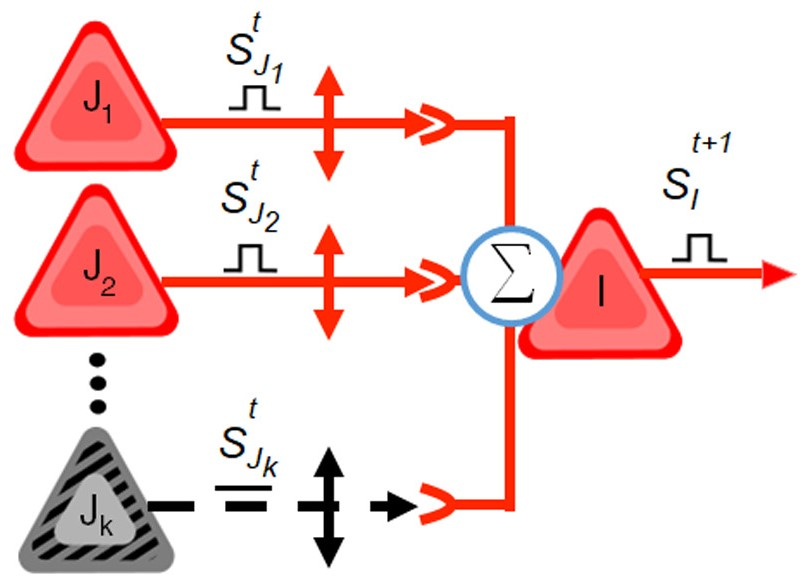
\includegraphics[width=\imsize]{reglaautomata}
	\caption[Regla para la propagación de la actividad neuronal en el modelo GH.]{Regla para la propagación de la actividad neuronal en el modelo GH. En este modelo, la activación de la neurona $i$ en el tiempo $t + 1$ está determinada por una suma ponderada de las contribuciones de todas las neuronas presinápticas activas, denotadas por $j_1$ y $j_2$, y multiplicadas por sus respectivas interacciones sinápticas $w_{ji}$. Esta suma ponderada debe superar el umbral $T$ para que la neurona $i$ se active en el siguiente paso de tiempo. Este proceso de actualización se repite para todas las neuronas inactivas $i$ en cada paso de tiempo. La Figura utiliza triángulos para representar las neuronas y líneas para indicar las interacciones sinápticas entre ellas. Las neuronas activas se muestran en color rojo, mientras que las neuronas inactivas se representan con triángulos grises punteados, tanto en el tiempo $t$ como en $t + 1$. Es importante resaltar que el término de suma en la regla de actualización refleja que el estado de la neurona $i$ en el tiempo $t + 1$ depende de la suma de las contribuciones de las neuronas $j_1$ a $j_n$.} 	\label{fig:reglaautomata}
\end{figure}



Por lo tanto,  las neuronas siempre exhiben un período refractario después de su activación, mientras que las neuronas en estado refractario tienen una probabilidad $r_2$ de retornar al estado quiescente en el siguiente intervalo de tiempo. La probabilidad de activación de una neurona en estado quiescente se define como el complemento del producto de las probabilidades de no activación a través de los distintos mecanismos \cite{diaz_similar_2021}. Un ejemplo de dos pasos de transición consecutivos se esquematiza en la \Cref{fig:modelopasos}. El modelo considera dos mecanismos de excitación: la excitación espontánea, que ocurre con una probabilidad $r_1$ y ejerce un papel de ruido en el sistema, y la excitación transmitida, que se produce de manera determinista.  En particular, una neurona se activará únicamente si se encuentra en estado quiescente y la suma de los pesos de las conexiones con sus vecinos activos supera el umbral $T$ (ver  \Cref{fig:modelopasos}). Los pesos $w_{ij}$ representan la distribución de pesos en el conectoma del C. elegans. Es importante destacar que el estado de cada neurona se actualiza una vez completada la actualización de toda la red.  Durante la dinámica temporal, la activación de una neurona ocurre con mayor frecuencia cuando la excitación entrante proveniente de sus vecinos activos más cercanos excede el umbral fijo $T$. En otras palabras, $T$ funciona como un parámetro umbral que regula la propagación de la actividad excitatoria entrante, de manera similar al potencial de acción en los modelos de neuronas de disparo \cite{rocha_homeostatic_2018}. Por otro lado, los parámetros $r_1$ y $r_2$ controlan la escala temporal de autoactivación y recuperación del estado excitado, respectivamente. Estos parámetros se ajustan en función del tamaño de la red, mientras que $T$ se establece como el parámetro de control del modelo.


\begin{figure}[ht]
	\centering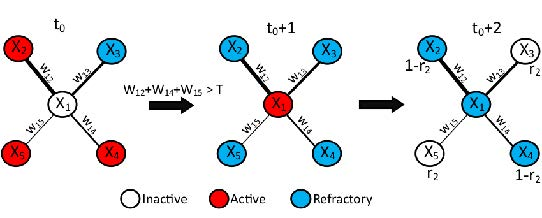
\includegraphics[width=\imsize]{modelopasos}
	\caption[Ejemplo de transiciones dinámicas en el modelo.]{Ejemplo de transiciones dinámicas en el modelo: en $t = t_0$ las neuronas activas son $x_2$,$x_4$ y $x_5$, que excitan $x_1$ en $t = t_0 + 1$, y luego ingresan al estado refractario con $t = t_0 + 2$, $x_3$ y $x_5$ se han recuperado y son susceptibles de excitarse nuevamente,
		mientras que $x_2$ y $x_4$ siguen siendo refractarios.} 	\label{fig:modelopasos}
\end{figure}




\subsection{Teoría de campo medio del modelo neuronal}

En sistemas reales, así como en autómatas celulares estocásticos, se busca comúnmente el estado de equilibrio promediado en el tiempo después de que hayan ocurrido los procesos iniciales rápidos, incluso en presencia de ciclos o aleatoriedad. En esta sección, se analiza el sistema neuronal del modelo previamente presentado que posee múltiples grados de libertad, utilizando herramientas de la mecánica estadística del equilibrio. Estas herramientas permiten describir directamente el estado de equilibrio del sistema en lugar de su evolución temporal. Aunque encontrar una solución exacta para este estado de equilibrio puede ser sumamente difícil e incluso imposible en muchos casos, se hará hincapié en una técnica de aproximación poderosa conocida como aproximación del campo medio, utilizada para describir sistemas con múltiples componentes que interactúan entre sí. La idea detrás de esta aproximación es considerar un solo elemento del sistema influenciado de manera promedio por el resto del sistema, y para lograrlo de manera correcta, es crucial calcular este promedio de manera autoconsistente \cite{bar-yam_dynamics_2003}.

Comenzando con la definición de la probabilidad de que una neurona se encuentre en un estado elemental específico $z^j \in \mathcal{E}=\left\{Q,E,R\right\}$  en el tiempo $t+1$   , podemos expresar esta probabilidad como:

\begin{equation}\label{eq:67}
	P\left(\xi_i(t+1)=z^j\right)=\sum_{\tilde{\mathbf{s}}_{\mathcal{N}(i)}\in\mathcal{S}_{\mathcal{N}(i)}}{P_t(\tilde{\mathbf{s}}_{\mathcal{N}(i)})}\prod_{i\in G}  {p_i\left(\xi_i(t+1)=z^j \mid  \bm{\xi}(t)\mid  \mathcal{N}^I(i) = \tilde{\mathbf{s}}\mid \mathcal{N}^I(i)   \right)}.	
\end{equation}

Al expresar la  \cref{eq:67}  en términos de la probabilidad de que la neurona $i$ esté excitada ($p_i^t \coloneqq  P_t(\tilde{s}=E)$),  en estado quiescente ($q_i^t \coloneqq  P_t(\tilde{s}=Q)$),  o en estado refractario ($r_i^t \coloneqq  P_t(\tilde{s}=R) =1-p_i^t-q_i^t$), se obtienen las siguientes ecuaciones:


\begin{align}
p_i^{t+1}&=q_i^t\left[r_1+\left(1-r_1\right)\Theta\left(\sum_{j=1}^{N}W_{ji}p_j^t-T\right)\right], \label{eq:56}\\
q_i^{t+1}&=q_i^t+r_2\left(1-p_i^t-q_i^t\right)-p_i^{t+1} \label{eq:57},
\end{align}

La \cref{eq:56} se deduce al considerar que  $q_i^t=1-p_i^t$, lo cual representa la probabilidad de que la neurona $i$ esté en estado quiescente en el momento $t$. El término entre paréntesis representa la probabilidad de que la neurona haga una transición al estado excitado, asumiendo que los sucesos en los que los vecinos de la neurona $i$ están excitados en el momento  $t$ son estadísticamente independientes.  Esta aproximación ha demostrado ser efectiva incluso en redes con bucles cortos significativos \cite{rocha_homeostatic_2018,larremore_predicting_2011}.


\subsubsection{Predicción de campo medio del punto crítico}

Pasemos ahora a la predicción del punto crítico mediante el campo medio. Obtener soluciones analíticas para  $p_i^t$ y $q_i^t$ en  las \cref{eq:56,eq:57} es difícil. Sin embargo, estudiando la solución de estado estacionario  ( $t \to\infty$ ) de la aproximación del campo medio, podemos encontrar una solución aproximada para el punto crítico $T_c$.  Para utilizar la aproximación del campo medio, seleccionamos una neurona particular $i$  y hallamos el campo efectivo (o campo medio) al que está expuesta.  Este campo se obtiene sustituyendo todas las variables por sus valores medios. Al establecer  $p_i^t = \left\langle p_i \right\rangle_t   = \bar{p}$ y $q_i^t =\left\langle q_i\right\rangle_t = \bar{q}$ en las ecuaciones \cref{eq:56,eq:57}, donde $\left\langle \cdot \right\rangle_t$ denota el valor esperado en el tiempo, y aproximando $W_i \coloneqq \sum_j W_{ji} \approx \left\langle W \right\rangle$,  con $\left\langle W \right\rangle = \sum_i W_i/N$ como la fuerza media de la red, obtenemos:
 

\begin{align}
	\bar{p}&=\bar{q}\left[r_1+\left(1-r_1\right)\Theta\left(\left< W\right>\bar{p}-T\right)\right], \label{eq:76}\\
	\bar{q}&=\bar{q}+r_2\left(1-\bar{p}-\bar{q}\right)-\bar{p} \label{eq:77},
\end{align}

Considerando la función Heaviside \[\left(\left< W\right>\bar{p}-T\right) = \begin{cases}
	1 & \text{si} T\leq T_c\\
	0 & \text{si } T>T_c
\end{cases}\] y $T_c=\left< W\right>\bar{p}$ como el valor del punto crítico, tras algunas manipulaciones se obtiene:

\begin{equation}\label{eq:78}
	\begin{aligned}
		T_c &= \left\langle W\right\rangle p_{-} =\frac{r_2 }{1+2r_2}\left\langle W\right\rangle ,	\\
		\bar{p}&=\bar{q}=\frac{r_2}{1+2r_2} \eqqcolon p_{-} &\ \text{cuando} \ T<T_c \\
		\bar{p} &= r_1\bar{q} = \frac{r_1r_2}{r_1+r_2+r_1r_2}\eqqcolon p_{+} &\ \text{cuando} \ T>T_c\\
		\end{aligned}
\end{equation}

como era de esperar, $p_{+} < p_{-}$, lo que implica que la actividad es alta cuando el umbral es bajo. Esta expresión es solo una aproximación del umbral crítico exacto. Sin embargo, la solución del campo medio proporciona un resultado razonable al considerar la variabilidad de los puntos críticos con la fuerza de la red  $\left\langle W \right\rangle$, como se ha observado numéricamente. Cabe destacar que $T_c$ depende del sistema nervioso considerado, ya que  $\left\langle W \right\rangle$ varía entre distintos sistemas nerviosos.





de tres estados.  A , q , y  R representan estados activos, inactivos y refractarios, respectivamente. Las flechas representan posibles transiciones con las tasas de transición indicadas. Las flechas abiertas indican que la tasa correspondiente es potencialmente dependiente del estado de la red, es decir, la actividad de las otras neuronas en la red, con funciones de tasa de activación  F y  g.
.

Ahora consideramos el modelo de campo neural con tres estados como un modelo genérico de una neurona en pico (\Cref{fig:estadoneuronas}), donde una neurona puede estar en un estado de pico activo (A), refractario (R) o inactivo (Q). Suponemos que las neuronas pueden sufrir las siguientes cuatro transiciones:


\begin{figure}[ht]
	\centering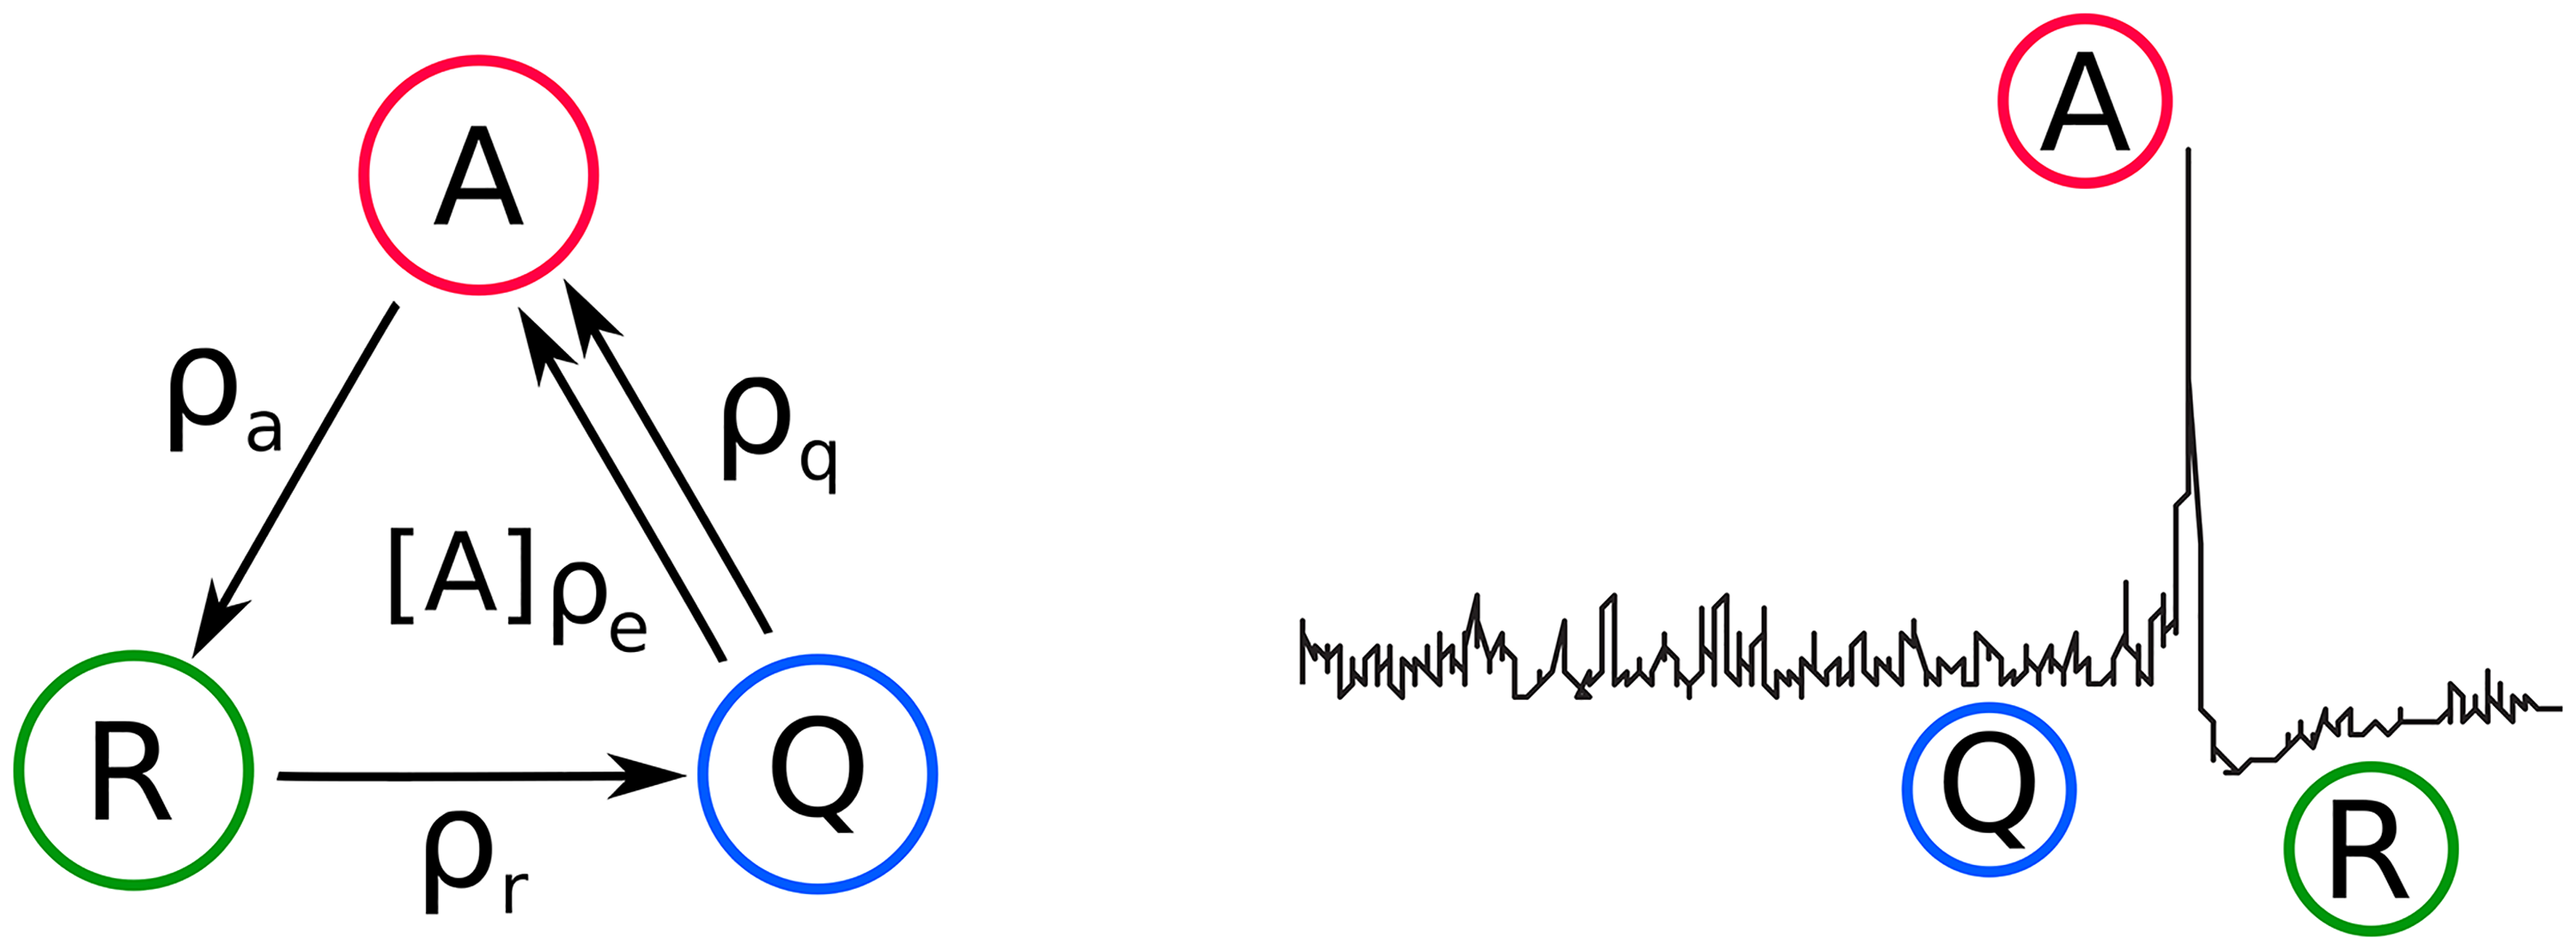
\includegraphics[width=\imsize]{estadoneuronas.png}
	\caption[Modelo neural de 3 estados quiescente-activo-refractario (QAR) .]{Modelo neural de 3 estados quiescente-activo-refractario (QAR). Las células en la retina en desarrollo se modelan con tres estados de actividad. Las células activas ( A ; rojo) disparan ráfagas de potenciales de acción, antes de volverse refractarias ( R ; verde) durante un período prolongado de tiempo. Las células inactivas ( Q ; azul) pueden estallar espontáneamente o pueden ser reclutadas en una ola por otras células activas.} 	\label{fig:estadoneuronas}
\end{figure}




\section{Discusión}
	
El presente capítulo se centró en la dinámica neuronal del cerebro de un organismo, destacando su naturaleza incesante y la exhibición constante de patrones espacio-temporales complejos de actividad coordinada, aun en la inactividad. Estas características de flexibilidad y adaptabilidad son fundamentales para enfrentar los desafíos ambientales relacionados con la supervivencia y la reproducción, y probablemente se originan debido a presiones evolutivas \cite{haimovici_dynamical_2016}. Se ha propuesto que estos patrones complejos emergen de la interacción entre la topología compleja del sistema nervioso del organismo y la dinámica de las neuronas individuales. En concreto, las redes neuronales en los cerebros de los organismos presentan características como longitudes de camino cortas, coeficientes de agrupamiento elevados y distribuciones de grado sesgadas. Estas arquitecturas altamente complejas influyen significativamente en los procesos que ocurren en las redes, lo que sugiere que el cableado neuronal puede ser crucial para la generación de oscilaciones y sincronización en el cerebro. Además de esta estructura altamente heterogénea y compacta, las redes neuronales también exhiben ruido intrínseco. Aunque las neuronas están sujetas a fluctuaciones térmicas que actúan como una fuente externa de ruido, la mayor parte de la variabilidad en los circuitos parece provenir de la actividad generada dentro de las propias redes neuronales. Esto implica que un enfoque estocástico es inevitable para abordar las actividades neuronales. A pesar de que inicialmente el ruido podría parecer perjudicial, en las redes neuronales puede tener un papel positivo al favorecer oscilaciones y sincronización, o al inducir resonancia estocástica.


El resultado más significativo de este capítulo es la formulación de un modelo de dinámica neuronal que exhibe todas las características mencionadas anteriormente. Este modelo integra una arquitectura de red basada en el conectoma del C. elegans, el cual posee propiedades topológicas complejas similares a las de un organismo real. Además, se incorpora una dinámica de red estocástica que representa el ruido intrínseco presente en las redes neuronales reales. Esta compleja interacción permite que la red exhiba estados de actividad irregular intrínsecamente generados, similares a la actividad coordinada que emerge del estado de reposo. La lógica computacional de este modelo se basa en la generación de eventos dinámicos locales y su comunicación global a través de la arquitectura de red característica. La generación de eventos se fundamenta en la acumulación de entradas en los nodos susceptibles, los cuales son excitados más allá de un umbral de entrada crítico. Después de su activación, los nodos pueden entrar en un período refractario durante el cual no pueden generar nuevos eventos, antes de regresar a un estado susceptible. Este ciclo básico de activación e inactividad es el sello distintivo de los medios excitables discutidos en el \cref{sec:mediosexcitables}. A pesar de su aparente simplicidad, este mecanismo básico puede dar lugar a dinámicas globales ricas cuando se combina con una organización de red heterogénea, como la proporcionada por el conectoma.

El modelo se implementa como un autómata celular estocástico, lo que lleva a la discusión de los autómatas celulares en este capítulo. Los autómatas celulares son sistemas dinámicos en grafos en los cuales los vértices tienen un conjunto finito de estados en tiempos discretos $t$. Los estados de los vértices cambian según una regla de actualización homogénea (la misma regla se aplica a todos los vértices) y local (la regla depende solo de una vecindad finita del vértice en cuestión). Aunque los autómatas celulares están definidos por reglas simples, pueden exhibir comportamientos dinámicos complejos a gran escala. De esta manera, ofrecen un mundo microscópico ficticio que reproduce la física correcta a una escala de granularidad gruesa, siendo la contrapartida del concepto físico de \textquote{campo}. Enfocándonos en las propiedades colectivas, es razonable buscar modelos mínimos que, incluso careciendo de reglas microscópicas realistas, puedan reproducir un comportamiento macroscópico relevante. Dadas las ventajas y características de los autómatas celulares, la dinámica de red del modelo se implementó en este marco matemático. Los autómatas celulares (AC) son una herramienta clave en la simulación de fenómenos naturales debido a su capacidad de proyectar y describir fenómenos simulados en un marco matemático adecuado. Además, describen una arquitectura masivamente paralela en la cual se puede implementar el simulador. El enfoque de los autómatas celulares es efectivo cuando la simplificación de las leyes microscópicas relacionadas con un fenómeno dado no es relevante a una escala macroscópica de observación. La mecánica estadística nos enseña que este hecho suele ser cierto para sistemas cuya complejidad surge de un comportamiento colectivo en lugar de aspectos distintivos de las interacciones microscópicas.


Por último, con el marco teórico presentado en este y los capítulos anteriores, estamos en condiciones de desarrollar los métodos y experimentos computacionales necesarios para confirmar o refutar la hipótesis de que la dinámica del cerebro de C. elegans inmovilizados opera cerca de un punto crítico. El siguiente capítulo presentará los resultados obtenidos al aplicar herramientas que permiten detectar firmas de criticidad tanto en experimentos con C. elegans reales como en la dinámica global que emerge del modelo. En el caso del modelo, realizaremos una caracterización cuantitativa de los regímenes dinámicos mediante el análisis estadístico del tamaño de los clústeres activos en el estado estacionario a lo largo del tiempo. Los clústeres se definen como conjuntos de nodos conectados que están activos simultáneamente, y su tamaño se calculará en cada paso de tiempo. Esta estrategia nos permitirá emplear las herramientas de la teoría de percolación que se presentaron en el \cref{sec:cap-percolacion}. En relación a los experimentos con gusanos inmovilizados, buscaremos propiedades de criticidad, como la presencia de cascadas espacio-temporales de actividad neuronal denominadas avalanchas neuronales.   La teoría de las transiciones de fase distingue diferentes tipos de dinámicas en los sistemas físicos. Se introducirán las herramientas estadísticas para detectar este tipo de fenómenos, y se discutirá cómo se aplicarán a los datos reales.   La detección de estas propiedades permitirá establecer un paralelismo entre el comportamiento de la dinámica cerebral del gusano real y las predicciones del modelo.

	
Concluyendo, Los anteriores capítulos sientan las bases teóricas necesarias para explorar la dinámica neuronal y su relación con la criticidad en el cerebro de C. elegans. El modelo de autómatas celulares se presenta como una herramienta valiosa para estudiar la aparición de patrones complejos de actividad coordinada en redes neuronales. La combinación de este modelo con herramientas de la teoría de percolación, la teoría crítica y la mecánica estadística nos permitirá identificar signos de criticidad, respaldando así la hipótesis de que el cerebro de C. elegans, incluso en estado inmovilizado, opera cerca de un punto crítico. Los resultados obtenidos en el siguiente capítulo serán esenciales para comprender mejor la dinámica cerebral y su relevancia en el procesamiento de información y la adaptabilidad en organismos más complejos.




















